\documentclass[10pt,twocolumn]{article}

\usepackage[letterpaper,margin=0.68in,columnsep=0.25in]{geometry}
\usepackage[T1]{fontenc}
\usepackage{lmodern}
\usepackage{microtype}
\usepackage{graphicx}
\usepackage{booktabs}
\usepackage{tabularx}
\usepackage{array}
\usepackage{rotating}
\usepackage{pdflscape}
\usepackage{dblfloatfix}
\usepackage{placeins}
\usepackage[font=small,labelfont=bf]{caption}
\usepackage{enumitem}
\usepackage{xcolor}
\usepackage{amsmath,amssymb}
\usepackage[numbers,sort&compress]{natbib}
\usepackage{url}
\usepackage[hidelinks]{hyperref}
\usepackage{balance}

\definecolor{linkblue}{HTML}{1F5A94}
\hypersetup{
  colorlinks=true,
  linkcolor=linkblue,
  citecolor=linkblue,
  urlcolor=linkblue,
  pdftitle={When Self-Modification Becomes Memory},
  pdfauthor={Yohei Nakajima},
  pdfsubject={Audited self-improving agent evaluation}
}

\setlength{\parindent}{1em}
\setlength{\parskip}{0pt}
\setlength{\emergencystretch}{1.5em}
\setlist{nosep,leftmargin=*}
\setcounter{secnumdepth}{2}
\setcounter{tocdepth}{2}
\providecommand{\tightlist}{\setlength{\itemsep}{0pt}\setlength{\parskip}{0pt}}
\providecommand{\pandocbounded}[1]{\resizebox{\linewidth}{!}{#1}}

\title{\vspace{-1.6em}\textbf{When Self-Modification Becomes Memory}\\
\large An Audited Comparison of Three Self-Improving Agent Substrates}
\author{Yohei Nakajima}
\date{July 2026}

\begin{document}
\maketitle
\vspace{-1.5em}

\begin{abstract}

Language-model agents can edit prompts, memories, tools, and code, but
self-improvement bundles five evidentiary propositions: retention,
expression, behavioral mediation, task improvement, and recursive
improvement. This study instruments the first four; the fifth requires
descendant-productivity evidence. We audit three
substrate-proposal-acceptance-interface configurations built around a
workspace, a procedure store, and an executable Pack. They share an
outer agent, a 28-task development curriculum, and cold-restart
evaluation on 19 held-out tasks. None of the three recorded lineages met
the frozen uplift criterion. The shared interface expressed retained
structure mainly as text; per-task item coverage ranged from 12\% to
100\%, and the actor had no retained invocation handle. Six
actor-visible-equivalent no-context arms issued byte-identical initial
requests per task yet differed on 7 of 19 tasks. A code audit found that
the nominal state-hidden ablation was not separable from cold at the
actor-visible boundary, so we retain its contrast as the frozen decision
rule and add pooled-six-control sensitivity; the null is unchanged.
Across nine configuration-family cells, an opaque sham scored below the
labeled ablation in five, above it in three, and tied once, so the
design cannot isolate possible sham interference from outcome spread.
Mechanism audits found policy-cap saturation, a common proposal-form
bottleneck, and vocabulary-associated selection of failure-derived
lessons. Two separately executed, outcome-blind model-coding passes
agreed that all 84 proposals shared one nonexecutable textual genre; one
coder also generated the proposals, and interpretive labels remain
exploratory. We contribute an expression profile, an equivalent
duplicates protocol, and a control ladder. In this harness, the
interface and acceptance mechanism are measurable components of the
self-improving system.

\end{abstract}

\section{Introduction}\label{introduction}

Language-model agents now edit their own prompts, memories, tools, and
source code, and the reported results are striking. STOP
\citep{zelikman2023stop} recursively improves its own improver. SICA
\citep{robeyns2025sica} raises its score on a SWE-bench Verified subset
from 17\% to 53\%. The Darwin Gödel Machine \citep{zhang2025dgm} more
than doubles SWE-bench performance across a branching archive of
self-modified descendants, and the Huxley-Gödel Machine
\citep{wang2025hgm} scores lineages by the productivity of their
descendants. These systems make self-modification easy to observe.
Self-improvement is a different empirical claim. A visible edit
establishes that the system changed itself. It does not establish that
the change was expressed at evaluation time, altered behavior, caused
better externally graded outcomes, or improved the system's capacity to
produce useful future changes.

We separate the statement that an agent improved itself into five
constructs: (1) \textbf{retention}, meaning persistent state changed;
(2) \textbf{expression}, meaning retained state reached the
evaluation-time policy; (3) \textbf{behavioral mediation}, meaning the
policy's trajectory or resource use changed; (4) \textbf{task
improvement}, meaning externally graded held-out performance rose beyond
matched controls and stochastic spread; and (5) \textbf{recursive
improvement}. These are distinct evidentiary propositions, not ordinal
performance levels. Retention and actor-visible expression can be
established descriptively; behavioral mediation, task improvement, and
recursive improvement generally require counterfactual or lineage
contrasts. This study instruments the first four and frames descendant
productivity as the required operationalization of the fifth.

We study those links in a heavily instrumented comparison of three
persistent self-modification substrates chosen for the breadth of their
native update surfaces: an arbitrary rewritable workspace, a
success-gated procedure store, and a governed, hash-pinned executable
ActiveGraph Pack. Each traversed the same ordered 28-task development
curriculum and then faced 19 disjoint held-out tasks across three
families after a cold restart. The design used external graders, four
arms, immutable receipts, hash-bound adjudication, and a frozen success
criterion. It also had one development lineage per configuration, one
model, and small task families. The orchestration and local ActiveGraph
family were self-built; SWE and Terminal used external official graders,
and every claim is scoped to the recorded harness. The frozen result is
null: none of the three recorded lineages met the criterion. This paper
explains why that null is informative and why several favorable and
unfavorable results inside our data dissolve under audit.

The audit measures mechanisms that recur across agent systems. First,
budgeted context is a common route from memory to later action. Under
that route, our three substrate-interface configurations delivered
between 12\% and 100\% of their declared retained items per task,
exposed no retained invocation handle in the actor-visible action
schema, and expressed native structural change to the acting policy
almost entirely as text. These percentages are within-substrate coverage
measures rather than comparable quantities of useful information.
Second, single-run task estimates can conceal substantial outcome
variability. Our six no-context labels issued byte-identical first
requests per task, seed included, and still differed on 7 of 19 tasks.
Their family-level means spanned 2/10 tasks (20.0 points) on SWE and 1/6
task (16.7 points) on Terminal; the continuous-score ActiveGraph span
was 21.3 points. Third, placebo context can change the computation it is
meant to control. On SWE, the Workspace evolved arm solved 8/10 tasks
and the sham solved 6/10, creating a 20-point evolved-minus-sham
contrast; the six equivalent no-context labels on the same ten tasks
already ranged from 6/10 to 8/10. Fourth, lexical retrieval and
append-only retention created observable selection and capacity effects.
A top-three retriever over-selected broad-vocabulary failure lessons,
and the Pack eventually blocked three consecutive updates at its policy
limit.

The shared reflection layer created a proposal-form bottleneck before
configuration-specific acceptance and native mutation. Two separately
executed outcome-blind model-coding passes using two model families over
all 84 update proposals assigned every proposal to the same
representational genre: natural-language, append-only, nonexecutable,
operational guidance with no specified activation. Interpretive fields
were less stable across coders and remain exploratory pending human
coding. One coder, Sol, was also the model that generated the proposals;
Terra supplied the different-family pass. The cross-model consistency
finding concerns the proposal layer. Native Workspace edits and Pack
source changes remained structurally real and heterogeneous.

The receipts cut in both directions. An apparent transfer success
involved an evolved SymPy pass matched by a no-context run that produced
essentially the same fix, while the retained SymPy lesson concerned a
different mechanism. An apparent retrieval failure scored exactly at the
minimum of six equivalent no-context runs. The one evolved result
outside its task's exact equivalent range was a regression in which
retained context accompanied a larger invalid intervention and the
ablation produced the smaller correct fix. A tie-aware conditional
exchangeability calculation expected 12/7 (1.71) outside-range results
and observed one, so the case is a mechanistic trace rather than a
population or chance detection. A case audit that can reject favorable
and unfavorable causal stories symmetrically is a minimum requirement
for interpreting individual trajectories.

Prior systems provide strong evidence for the forms of optimization they
measure. Table 6 records which studies report held-out transfer,
mechanism ablations, sham retained state, independent evolution runs,
byte-identical initial-request duplicates, immutable receipts, and
descendant productivity. We do not reinterpret their reported gains
through our experiment. Under our controls, our apparent gains
dissolved. Applying the same instruments in independent systems is a
concrete next test.

This paper contributes six reusable instruments and observations:

\begin{enumerate}
\def\labelenumi{\arabic{enumi}.}
\tightlist
\item
  a five-construct decomposition separating retention, expression,
  behavioral mediation, task improvement, and recursive improvement;
\item
  an \textbf{expression profile} measuring storage reach,
  eligible-payload reach, semantic-unit reach, selection adaptivity, and
  execution reach;
\item
  an \textbf{equivalent duplicates} protocol that creates task-level
  empirical dispersion references from executions with byte-identical
  initial requests;
\item
  a \textbf{control ladder} organizing eight control designs by the
  nuisance they address and the claims they license;
\item
  mechanism checks for \textbf{failure-memory stickiness}, capacity
  saturation, and common-template reflection-proposal homogenization;
  and
\item
  a receipt-bound compact release with graders, requests, artifacts, and
  an adjudication ledger; complete trajectory traces remain in a
  separately gated archive pending disclosure review and deposit.
\end{enumerate}

The scope is a within-study diagnostic demonstration. It does not supply
a population estimate, a universal architecture ranking, or a universal
auditability-expressivity law. The expression bottleneck was created by
the implemented common interface, and that fact is central to the
result. The reflection template determined what could be proposed, the
acceptance gate determined what survived, the retriever and adapter
determined what was expressed, and the execution stack determined what a
score could mean. The interface and the acceptance mechanism are part of
the self-improving system.

\begin{figure*}[!t]
\centering
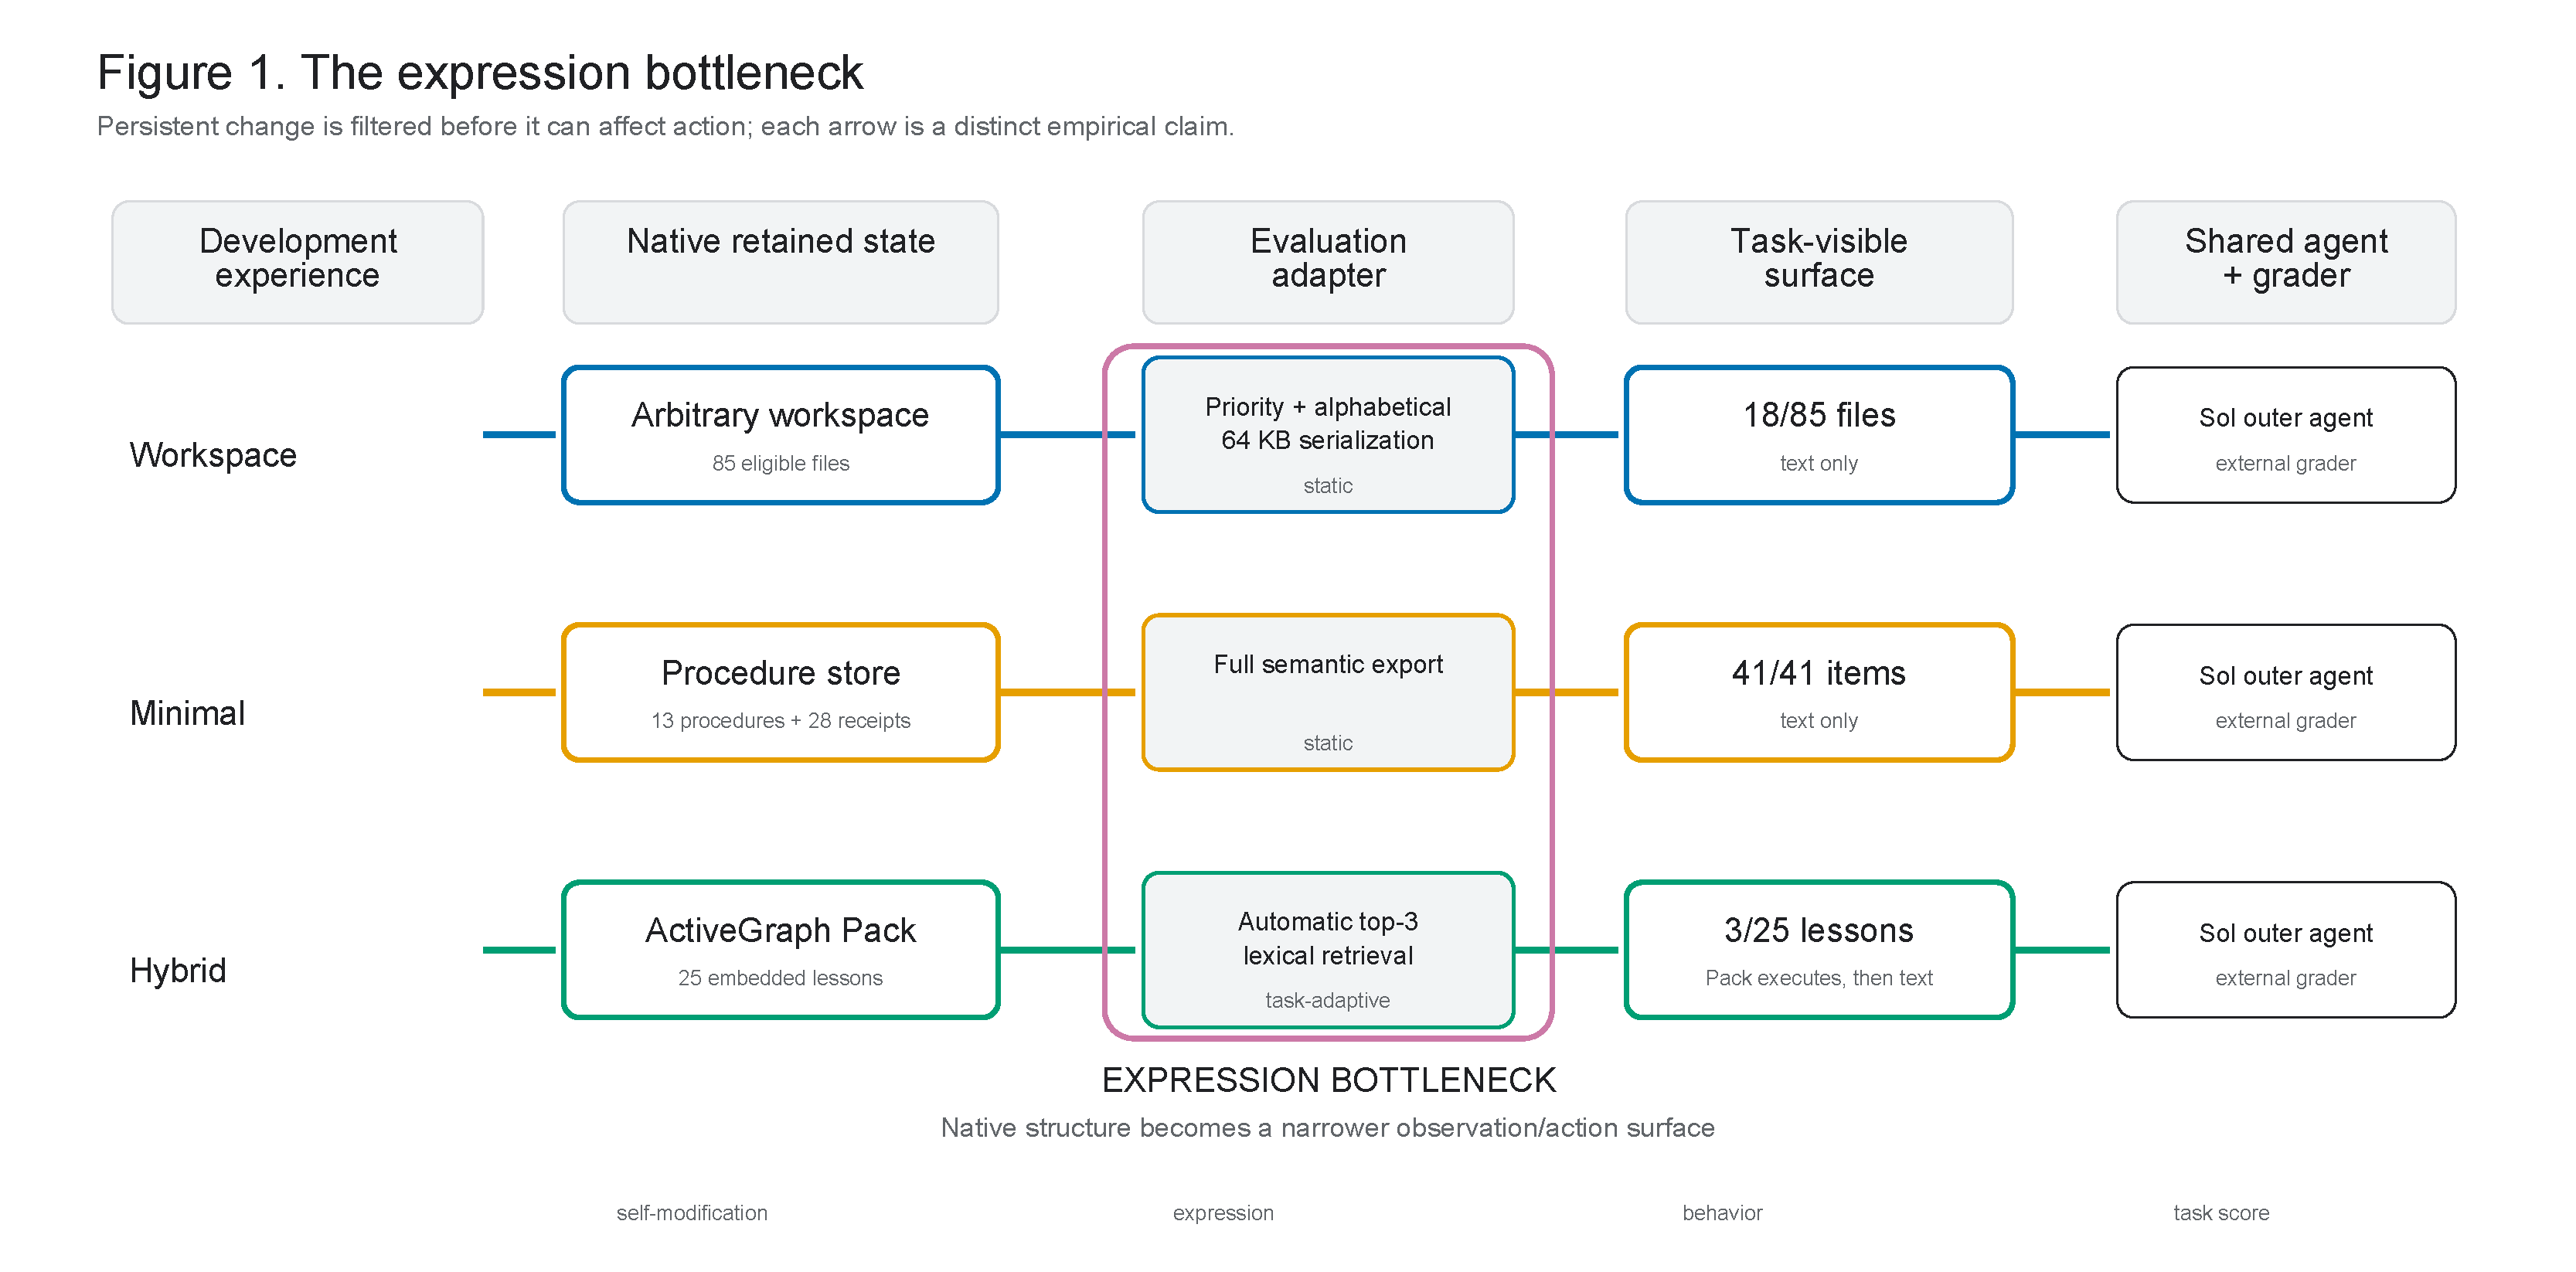
\includegraphics[width=0.82\textwidth]{figures/pdf/figure-1-expression-bottleneck.pdf}
\caption{\textbf{The expression bottleneck.} The study separates
retention, expression, behavioral mediation, task improvement, and
recursive improvement. Retention is necessary but does not identify
later score improvement or recursive self-improvement. The bold
bottleneck is the implemented adapter boundary. It does not imply that
all auditable interfaces reduce expressivity.}
\label{fig:1}
\end{figure*}

\section{Measurement framework}\label{measurement-framework}

Let \(R_i^t\) denote retained state for configuration \(i\) after
development generation \(t\). Let \(A_i(R_i^t, x)\) be the evaluation
adapter for task \(x\), \(O_i^t(x)\) the observation and action surface
emitted by the adapter, \(\pi(O_i^t(x), x)\) the induced acting policy,
\(Y_i^t(x)\) the external task score, and \(M_i^t\) the productivity of
the process that creates useful descendants. The five constructs
correspond to different comparisons:

\begin{enumerate}
\def\labelenumi{\arabic{enumi}.}
\tightlist
\item
  Retention: \(R_i^{t+1} \ne R_i^t\).
\item
  Expression: \(O_i^{t+1}(x) \ne O_i^t(x)\).
\item
  Behavioral mediation: the induced policy trajectory changes.
\item
  Task improvement: expected external score increases beyond matched
  controls and relevant outcome spread.
\item
  Recursive improvement: the productivity \(M_i^t\) of generating useful
  descendants increases.
\end{enumerate}

This decomposition prevents evidence from moving silently between
levels. The five propositions have different logical status and need not
move together. A new file establishes retention. A serialized lesson
establishes possible expression. A changed trace establishes behavioral
mediation. An external score contrast supports task improvement.
Recursive improvement is the construct; descendant productivity is its
operationalization. It requires evidence that earlier changes improved
later update production.

\subsection{Expression profile}\label{expression-profile}

A single byte ratio cannot compare heterogeneous stores. Minimal's
complete SQLite state is mostly provenance, while its semantic export is
small. Workspace bytes mix source, tests, instructions, and records.
Hybrid executes a Pack query before the actor, so direct byte delivery
omits runtime activation. We therefore report five structured axes:

\begin{enumerate}
\def\labelenumi{\arabic{enumi}.}
\tightlist
\item
  \textbf{storage reach}: unique bytes copied into the initial
  actor-visible context divided by bytes in a declared canonical
  serialization of the complete frozen retained-state snapshot;
\item
  \textbf{eligible-payload reach}: those copied bytes divided by the
  canonical retained byte spans admitted by the adapter's frozen
  eligibility rule;
\item
  \textbf{semantic-unit reach}: declared substrate-native retained items
  surfaced per task, plus their union across the probe, divided by the
  frozen item inventory;
\item
  \textbf{selection adaptivity}: whether selection is explicitly
  conditioned on task input, accompanied by the per-task-to-probe-union
  coverage expansion; and
\item
  \textbf{execution reach}: whether retained code runs automatically and
  how many retained invocation handles appear in the actor-visible
  action schema.
\end{enumerate}

Semantic units are files for Workspace, typed procedures, capabilities,
or receipts for Minimal, and lessons for Hybrid. The unitization rule
and item types are frozen before evaluation. A Workspace file counts
once when any bounded prefix of that file reaches the actor;
completeness is reported separately. These ratios measure coverage
within one substrate and must not be used to compare quantities of
useful information across substrates. The coverage-expansion gap
measures selection turnover; it does not by itself show that selection
is relevant or beneficial. Interfaces without byte-copy semantics should
report the byte axes as not applicable and declare a proxy rather than
force a ratio.

The expression profile is diagnostic rather than ordinal. Greater reach
can increase useful transfer, interference, cost, or all three.

\subsection{Control ladder}\label{control-ladder}

The control ladder organizes controls by the nuisance they address and
the inference they license. Rungs 3 through 6 are alternative payload
controls, not a monotonic sequence in which every higher number
dominates every lower number.

\begin{table*}[t]
\caption*{\textbf{Control ladder.} Payload controls 3--6 are alternatives rather than a monotonic sequence.}
\centering\scriptsize
\begin{tabularx}{\textwidth}{@{}p{0.15\textwidth}X X@{}}
\toprule
\textbf{Control} & \textbf{Intervention and held-fixed variables} & \textbf{Licensed inference}\\
\midrule
1. Cold floor & Same model, task, harness, and budget; no lineage & Model-and-harness floor\\
2. State-hidden ablation & Same developed lineage and evaluation stack; learned state hidden; a distinct actor-visible channel is required & Effect of enabling retained state only when that distinct channel is verified\\
3. Opaque byte-size sham & Seeded opaque text; report byte ratio and token load & Sensitivity to opaque payload of recorded size\\
4. Token-matched neutral sham & Match tokenizer, position, and count with a preregistered corpus and blinded relevance screen & Payload effect after equalizing first-call token load\\
5. Semantic sham & Plausible units from disjoint task families under blinded relevance screening & Sensitivity to screened-unrelated guidance\\
6. Structure-preserving sham & Preserve count, schema, and token budget while permuting content or metadata & Sensitivity to retained structure apart from its original mapping\\
7. Equivalent duplicates & Byte-identical initial request, model, seed field, task image, harness, and budgets; later trajectories may diverge & Observed within-task execution dispersion\\
8. Native-interface ablation & Hold state, task, model, and budgets fixed while toggling native execution & Effect of the native execution path with recorded downstream changes\\
\bottomrule
\end{tabularx}
\end{table*}

The present study separably implements rungs 1, 3, and 7. It records the
lineage state hash required by rung 2, but the cold-ablation adapters
validate and then suppress that state without exposing a lineage-derived
channel to the actor. Cold and cold ablation therefore collapse at the
actor-visible intervention boundary. Rung 2 is not separably implemented
here. The other rows are operational specifications for follow-up
designs rather than empirical controls claimed here.

\section{Study design}\label{study-design}

All three configurations used the same \texttt{gpt-5.6-sol} outer coding
agent, brokered tool protocol, task ceilings, grader boundary, and
common reflection step. Accordingly, the experiment compares three
proposal, acceptance, retention, and interface configurations downstream
of one shared textual proposal generator. It does not compare
unconstrained native self-modification processes. The configurations
differed in retained state:

\begin{itemize}
\tightlist
\item
  \textbf{Workspace v1.2} could rewrite and retain an arbitrary
  workspace tree.
\item
  \textbf{Minimal v2} stored every scalar receipt and promoted only
  successful experiences as procedures or deterministic capabilities.
\item
  \textbf{Hybrid Packs} used a model-authored, tested, hash-pinned
  ActiveGraph Pack to store and retrieve lessons.
\end{itemize}

The native mutation units differ in breadth. The score comparison
concerns their implemented common interface and does not order their
native ceilings.

Each configuration traversed the same 28-task development curriculum: 20
SWE-bench Verified issues, six Terminal-Bench 2 tasks, and two local
Ouro-ActiveGraph-50 systems. Evaluation used 19 disjoint held-out tasks:
ten SWE-bench Verified issues, six Terminal-Bench 2 tasks, and three
Ouro-ActiveGraph-50 systems. SWE and Terminal used official binary
verifiers. The ActiveGraph family used normalized scores from 50 sealed
checks. The local benchmark and the Hybrid Pack both use ActiveGraph
technology, creating a structural author-built overlap. The sealed
checks and the unfavorable Hybrid ActiveGraph result, -10.0 points
versus its labeled ablation, mitigate simple directional bias but do not
remove that conflict.

For each configuration and held-out task, the study ran four arms:

\begin{itemize}
\tightlist
\item
  \textbf{evolved}, with retained development state enabled;
\item
  \textbf{cold ablation}, with the same lineage hash validated and
  learned state hidden;
\item
  \textbf{sham}, with a seeded opaque artifact intended to approximate
  the evolved context size; and
\item
  \textbf{cold}, with no development state.
\end{itemize}

Source inspection after Round 1 confirmed that cold and cold ablation
have the same task, model, seed field, tools, workspace, system
instructions, empty retained-context field, and later actor-visible tool
protocol. The hidden lineage hash is validated for cold ablation but
never reaches the actor. The frozen primary estimand, paired
\texttt{evolved\ -\ cold\ ablation}, is therefore an evolved contrast
against one labeled draw from the six actor-visible-equivalent
no-context arms rather than a separable matched-lineage intervention. We
keep that contrast as the frozen decision rule and report pooled-six and
leave-the-matched-ablation-out sensitivities in Section 4.

The frozen rule required benefit over ablation and sham, a nominal 95\%
task-resampling interval above zero in at least two families including
SWE or Terminal, valid cold reload, and no material development
regression. This was an operational decision rule for the recorded probe
rather than a claim of population-level interval coverage.

The information boundary excluded hidden tests, expected outputs,
private cases, grader logs, and oracle artifacts from lineage state.
Each accepted generation produced an immutable directory whose manifest
bound architecture, parent run, development experience, artifact size,
and hash. Evaluation occurred after cold reload. The study specification
is \path{../research/local_study.json}, SHA-256
\texttt{8313d219\allowbreak{}71452704\allowbreak{}893200d2\allowbreak{}022718fe\allowbreak{}ca985142\allowbreak{}ae32fe7d\allowbreak{}16932d34\allowbreak{}a0e0d581},
committed with frozen status at study commit
\texttt{55984389\allowbreak{}4578141d\allowbreak{}fbd39b7b\allowbreak{}ae2246db\allowbreak{}76e57bde}
on 2026-07-17T18:30:38-07:00. The compact release does not preserve an
independently witnessed timestamp for the first development call, so we
call this a frozen study specification and decision rule rather than an
externally registered preregistration. The manuscript package reviewed
in Round 1 was commit
\texttt{8bdff502\allowbreak{}cc08be96\allowbreak{}8b21bbe5\allowbreak{}ebf177d4\allowbreak{}9879a0fb}.

The study completed 84 development attempts and 228 held-out attempts.
Failed attempts remained in the denominator. Six SWE runs reached the
frozen 3,600-second task limit. Six Terminal agents reached the
1,800-second limit, and completed verifiers returned zero. One
ActiveGraph grader contradicted a receipt-bound parsable submission; one
sealed grader-only retry of the hash-identical artifact recovered 24/50.
No model attempt was rerun and no raw row was rewritten. The
adjudication index binds the raw report, datasets, changed analytical
row, and evidence by SHA-256.

Scores remain separate by family. Nominal 95\% descriptive
task-resampling intervals use 10,000 deterministic percentile-bootstrap
draws. Each draw resamples the paired per-task arm differences jointly
with replacement. With one lineage and ten, six, and three held-out
tasks, no frequentist coverage is asserted. The three-task ActiveGraph
interval is especially discrete and unstable.

\section{Frozen outcome rule and pooled-control sensitivity}\label{frozen-outcome-rule-and-pooled-control-sensitivity}

None of the three recorded lineages met the frozen uplift criterion.
Table 1 reports the binary families as fractions and percentages. For
context, the six equivalent no-context labels ranged from 6/10 to 8/10
on SWE and from 4/6 to 5/6 on Terminal despite byte-identical initial
requests within each task.

\begin{table*}[t]
\caption{Frozen held-out outcomes. Intervals are nominal descriptive task-resampling intervals; [0, 0] intervals are degenerate observed contrasts, not population certainty.}
\label{tab:outcomes}
\centering\tiny
\setlength{\tabcolsep}{3pt}
\begin{tabular}{@{}llrrrrr@{}}
\toprule
\textbf{Family} & \textbf{Configuration} & \textbf{Evolved} & \textbf{Labeled ablation} & \textbf{Evolved--ablation [interval]} & \textbf{Sham} & \textbf{Evolved--sham}\\
\midrule
SWE (10) & Workspace & 8/10 & 8/10 & 0/10 [0, 0] pp & 6/10 & +2/10\\
 & Minimal & 7/10 & 6/10 & +1/10 [-20, +40] pp & 7/10 & 0/10\\
 & Hybrid & 8/10 & 7/10 & +1/10 [0, +30] pp & 8/10 & 0/10\\
Terminal (6) & Workspace & 5/6 & 4/6 & +1/6 [0, +50] pp & 3/6 & +2/6\\
 & Minimal & 3/6 & 5/6 & -2/6 [-66.7, 0] pp & 4/6 & -1/6\\
 & Hybrid & 4/6 & 4/6 & 0/6 [0, 0] pp & 4/6 & 0/6\\
ActiveGraph (3) & Workspace & 82.7\% & 100.0\% & -17.3 [-52, 0] pp & 96.0\% & -13.3 pp\\
 & Minimal & 96.7\% & 88.0\% & +8.7 [-10, +36] pp & 100.0\% & -3.3 pp\\
 & Hybrid & 82.7\% & 92.7\% & -10.0 [-40, +10] pp & 82.7\% & 0.0 pp\\
\bottomrule
\end{tabular}
\end{table*}

Intervals equal to {[}0, 0{]} are degenerate because every paired task
difference was zero; they do not imply population-level certainty. The
labeled ablation column preserves the frozen comparison even though
source inspection later showed that it was one no-context draw rather
than a separable lineage intervention.

The pooled-six sensitivity recomputes the descriptive mean contrast
against all actor-visible-equivalent no-context labels. In Workspace,
Minimal, and Hybrid order, the evolved-minus-pooled deltas are +6.7,
-3.3, and +6.7 points for SWE; +11.1, -22.2, and -5.6 points for
Terminal; and -9.9, +4.1, and -9.9 points for ActiveGraph. Leaving each
configuration's labeled ablation out of its reference gives +8.0, -6.0,
and +6.0; +10.0, -20.0, and -6.7; and -8.4, +3.2, and -9.9 points,
respectively. None changes the frozen no-uplift decision. The exact
nine-cell calculation is
\path{data/generated/equivalent-control-sensitivity.csv}.

The table and sensitivity establish persistent evaluation after
development and the absence of frozen uplift. They do not explain
whether retained state was available, whether it changed behavior, or
whether visible contrasts exceeded outcome variability. Sections 5
through 7 audit those links.

\section{Expression bottleneck}\label{expression-bottleneck}

All three substrates created cold-loadable state:

\begin{table}[t]
\caption{Retained state after 28 development tasks.}
\label{tab:retention}
\centering\scriptsize
\begin{tabularx}{\columnwidth}{@{}lrrX@{}}
\toprule
 & \multicolumn{2}{c}{\textbf{Accepted after}} & \\
\cmidrule(lr){2-3}
\textbf{Substrate} & \textbf{Pass} & \textbf{Fail} & \textbf{Final retained product}\\
\midrule
Workspace & 13 & 12 & 429,731-byte workspace\\
Minimal & 13 & 0 & 13 procedures, 0 capabilities, 28 receipts\\
Hybrid & 15 & 10 & 25 lessons; 62,506-byte Pack\\
\bottomrule
\end{tabularx}
\end{table}

These receipts establish retention. The expression profile shows what
could reach later behavior:

\begin{table*}[t]
\caption{Expression profile. Coverage ratios are within-substrate and do not compare useful information. Workspace counts a bounded partial-file prefix once and reports completeness separately.}
\label{tab:expression}
\centering\tiny
\setlength{\tabcolsep}{3pt}
\begin{tabularx}{\textwidth}{@{}lrrXXX@{}}
\toprule
\textbf{Substrate} & \textbf{Storage} & \textbf{Eligible} & \textbf{Semantic: task; union} & \textbf{Selection; expansion} & \textbf{Execution: automatic; handles}\\
\midrule
Workspace & 14.9\% & 25.9\% & 18/85 (21.2\%); 18/85 & static; 0 pp & none; 0, retained tools hidden\\
Minimal & 1.35\% & 99.6\% & 41/41 (100\%); 41/41 & static; 0 pp & none; N/A, 0 executable units\\
Hybrid & 4.0\% mean & 17.1\% mean & 3/25 (12\%); 17/25 (68\%) & task-conditioned; 56 pp turnover & automatic Pack query; 0 handles\\
\bottomrule
\end{tabularx}
\end{table*}

Minimal supplies the decisive counterexample to storage reach as a
sufficient metric. Its database and provenance artifacts were large,
giving 1.35\% storage reach, while the adapter exported all declared
semantic units. Those 41 units comprised 13 procedures and 28 receipts.
None was a deterministic capability. The byte numerators and
denominators are Workspace 64,000/429,731 storage and 64,000/247,411
eligible payload; Minimal 24,767/1,839,823 and 24,767/24,865; and Hybrid
mean 10,677/266,265 and 10,677/62,319.

Workspace exposed 17 complete files and a bounded prefix of an
eighteenth. Under the frozen semantic-unit rule, a file counts once when
any bounded prefix reaches the actor, yielding 18/85; completeness is
reported separately. All post-priority files came from the
alphabetically early \texttt{\_development/} directory, and the actor
could not invoke retained tools. Minimal delivered the same complete
export to every task. Hybrid alone selected different learned units by
task: three of 25 per task and 17 of 25 across the probe. Its Pack
executed a retrieval before each task, while the actor received only the
returned text and could not call the Pack interactively.

The common adapter therefore narrowed each native substrate in a
different way. Workspace was truncated and static. Minimal was
semantically complete and static. Hybrid used task-conditioned selection
with 56 points of probe-union coverage expansion. No actor-visible
action schema contained a retained invocation handle. Minimal had no
retained executable unit, while Workspace and Hybrid retained executable
material that the actor could not invoke on demand. This supports an
expression bottleneck in the implemented interface. A general
auditability-expressivity tradeoff remains a hypothesis for a future
interface intervention.

\begin{figure*}[!t]
\centering
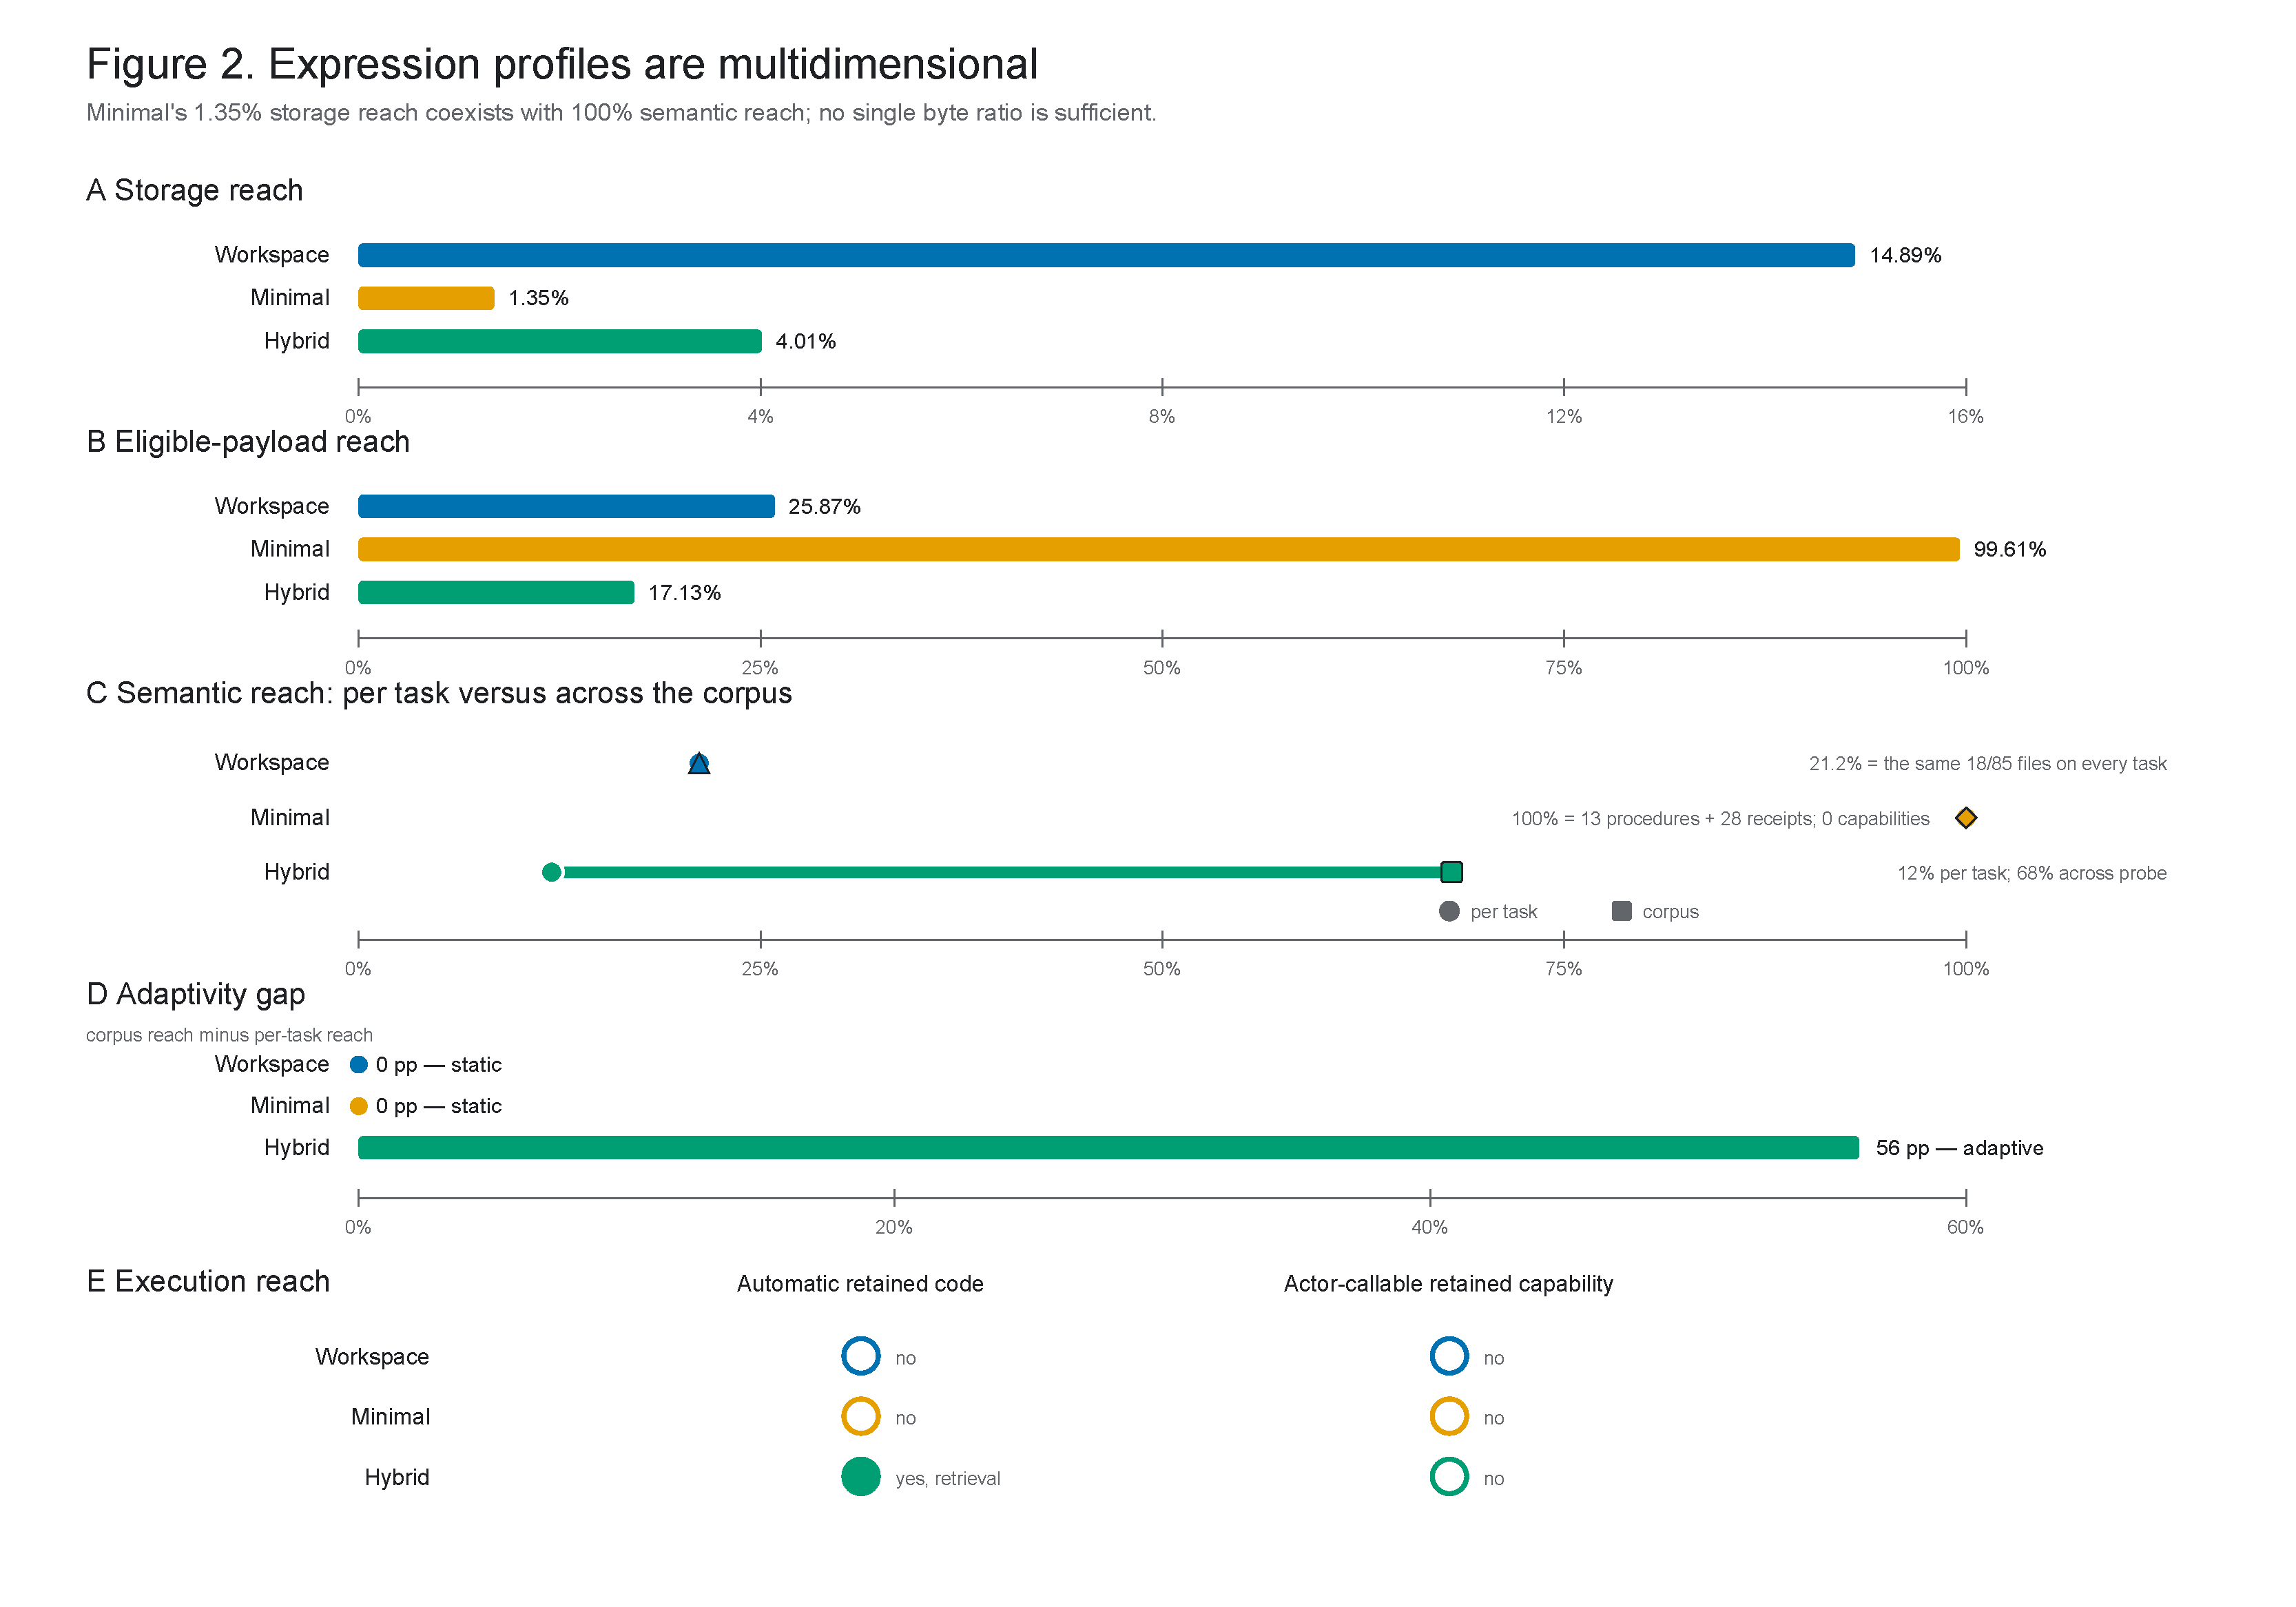
\includegraphics[width=0.85\textwidth]{figures/pdf/figure-2-expression-profile.pdf}
\caption{\textbf{Expression is a profile.} Five axes are reported:
storage reach, eligible-payload reach, semantic coverage with per-task
and probe-union submeasures, selection adaptivity, and execution reach
with automatic and actor-visible submeasures. Percentages are
within-substrate coverage measures and do not compare quantities of
useful information. Minimal's 41 declared units are 13 procedures and 28
receipts; none is executable. Hybrid conditions top-three selection on
task text, exposing three of 25 lessons per task and 17 across the
probe. Its Pack runs automatically in the adapter and supplies no
on-demand actor-visible invocation handle.}
\label{fig:2}
\end{figure*}

\section{Equivalent duplicates and control interference}\label{equivalent-duplicates-and-control-interference}

The six no-context labels were Workspace cold, Workspace ablation,
Minimal cold, Minimal ablation, Hybrid cold, and Hybrid ablation. For
each task, their first model requests were byte-identical, including
seed. Their outcomes varied on 7 of 19 tasks. The remaining 12 tasks
were stable: ten fixed passes and two fixed failures. Later model
sampling, tool outputs, timing, and trajectories were uncontrolled
execution variation, but actor-visible task, model, seed field, tools,
workspace, system instructions, retained-context field, and tool
protocol were the same. Three of these six labels are also the labeled
ablation comparators in Table 1, so the dispersion reference and frozen
comparator are overlapping rather than independent samples.

\begin{table*}[t]
\caption{Equivalent duplicate-execution dispersion and planning diagnostics. Neither planning quantity is a decision threshold.}
\label{tab:duplicates}
\centering\scriptsize
\begin{tabular}{@{}lrrrrr@{}}
\toprule
\textbf{Family} & \textbf{Tasks} & \textbf{Tasks variable across six labels} & \textbf{ICC(1,1)} & \textbf{Maximum pair gap} & \textbf{Continuous-approx. planning}\\
\midrule
SWE & 10 & 3 & 0.72 & 2/10 (20.0 pp) & 30.7 pp\\
Terminal & 6 & 2 & 0.66 & 1/6 (16.7 pp) & 45.1 pp\\
ActiveGraph & 3 & 2 & 0.31, unstable & 21.3 pp & 28.7 pp\\
\bottomrule
\end{tabular}
\end{table*}

The one-way random-effects ICC treats tasks as targets and the six named
no-context labels as exchangeable single replicate executions on the
observed score scale. It is a descriptive repeatability coefficient, and
the three-target ActiveGraph value is especially unstable. The
design-sizing diagnostic is \((1.96 + 0.842)\widehat{SE}\), using a
two-sided nominal \(\alpha=0.05\), 80\% power, and the within-task
variance across the six equivalent labels. It is a continuous normal
approximation for a paired mean contrast. On the binary families it does
not represent an attainable observed score increment. The three-task
ActiveGraph value is illustrative only and must not be used to interpret
the continuous-score spread as a stable power estimate. Neither planning
quantity is a decision threshold.

All discriminative variation in the no-context probe was concentrated in
seven tasks that changed outcome under equivalent requests. Stable tasks
still provide one-sided opportunities: fixed passes can expose
regressions and fixed failures can expose gains. Minimal's evolved
failure on \texttt{scikit-learn\_\_scikit-learn-13124}, against six
equivalent passes, was the only one of 57 evolved configuration-task
results outside an exact task-specific equivalent range. Under a
tie-aware conditional exchangeability calculation, the expected count is
12/7 (1.71): 1/7 among 36 cases on stable control tasks and 11/7 among
21 cases on variable control tasks. The observed count was one and
therefore supplies no positive chance detection. Method and family
breakdown are recorded in
\path{data/generated/outside-range-exchangeability.json}.

The maximum of the 15 absolute pairwise label-mean gaps is reported for
each family. The 15 values are dependent functions of six labels, and
the labels are not randomized evolution replications. The maximum is a
descriptive dispersion reference rather than a significance threshold.

The sham comparison exposes a second control problem. Workspace SWE
evolved minus sham was +2/10 tasks (+20.0 points) because the evolved
and ablation arms each solved 8/10 tasks while the opaque sham solved
6/10; equivalent no-context labels on the same tasks also ranged from
6/10 to 8/10. On Terminal, Workspace evolved minus sham was +2/6 tasks
(+33.3 points) because evolved solved 5/6, ablation solved 4/6, and sham
solved 3/6; equivalent labels on those tasks ranged from 4/6 to 5/6. The
SWE sham family score fell within the equivalent-label range, at 6/10
against 6/10 to 8/10. The Terminal sham fell below all six equivalent
family means, at 3/6 against 4/6 to 5/6. With six dependent draws, a
seventh observation below the observed minimum is consistent with
interference and does not establish it. The sham consumed approximately
1.88 to 2.43 times as many incremental first-call tokens per byte as
evolved context, depending on configuration. Its context bytes exactly
matched evolved context for Workspace and Minimal. For Hybrid, the
6,093-byte sham was 56\% to 58\% of the mean evolved context across
families. Byte matching therefore controlled artifact size while leaving
tokenization, semantic load, and interference uncontrolled for Workspace
and Minimal; Hybrid also retained a substantial byte-size mismatch.

\begin{figure*}[!t]
\centering
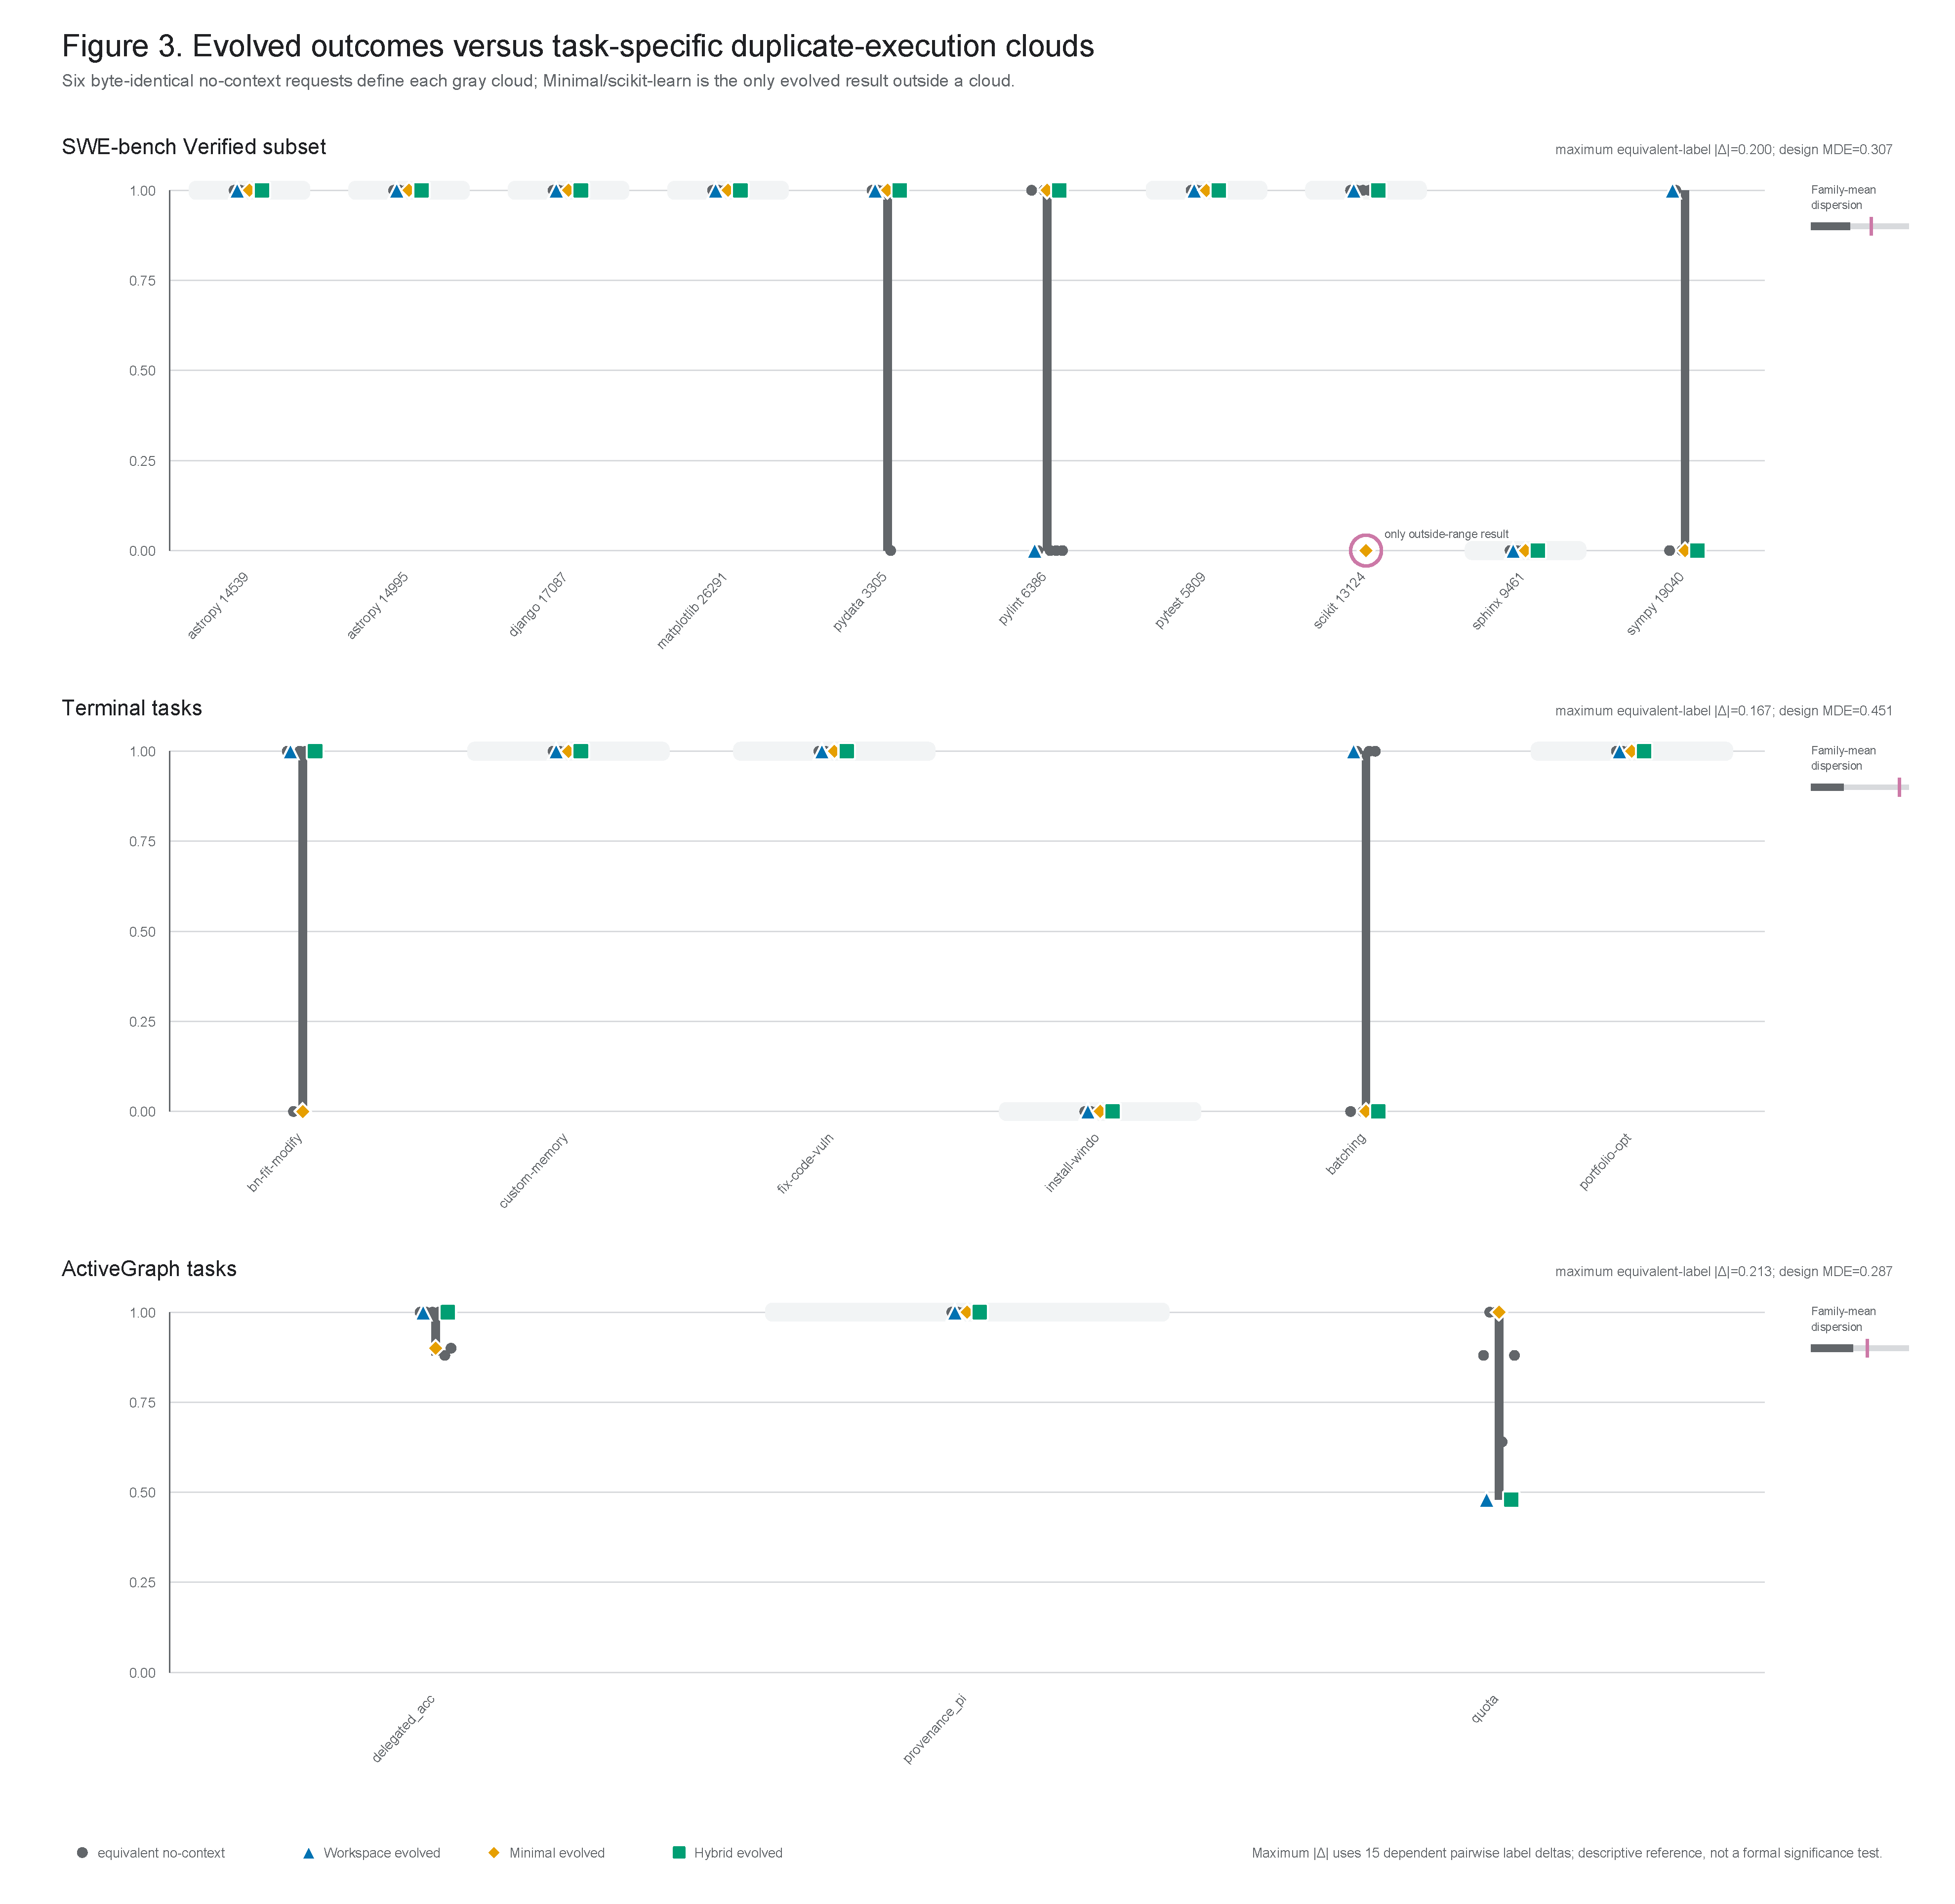
\includegraphics[width=0.92\textwidth]{figures/pdf/figure-3-task-level-noise.pdf}
\caption{\textbf{Task-level initial-request duplicate spread.} For each
of 19 tasks, gray points show six no-context outcomes generated from
byte-identical initial model requests; colored marks show the three
evolved outcomes. Later trajectory inputs may diverge. Seven tasks
varied under the duplicate executions and 12 were stable.
Minimal/scikit-learn is the only evolved configuration-task outcome
outside the observed duplicate-execution range. The bar is the maximum
of 15 dependent absolute pairwise label-mean gaps and is descriptive
rather than a formal significance threshold. Neither the bar nor the
planning diagnostic is a decision threshold.}
\label{fig:3}
\end{figure*}

\section{Mechanism audits}\label{mechanism-audits}

\subsection{Failure-memory stickiness}\label{failure-memory-stickiness}

Hybrid retained 25 lessons, including 15 from passing development
attempts and ten from failed attempts. Across 19 held-out tasks, the
top-three retriever filled 57 slots. Failure-derived lessons occupied
37/57 slots (64.9\%) despite forming 10/25 of the corpus (40\%). Two
failed Pylint lessons occupied 22/57 slots (38.6\%). Only 17/25 lessons
were ever retrieved, and 5/57 slots shared a repository prefix with the
held-out task.

The implemented ranker counted set overlap between task words and an
index containing suite, task identifier, title, scope, and trigger
terms. Failure-derived lessons had broader indexed vocabularies. The raw
enrichment, 37/57 retrieval slots from 10/25 failure-derived lessons, is
the total association. Indexed vocabulary correlated with retrieval
count within passing lessons (\(\rho=0.743, n=15\)) and failed lessons
(\(\rho=0.763, n=10\)). In the descriptive regression
\texttt{retrievals\ \textasciitilde{}\ indexed\ vocabulary\ +\ failure\ flag},
vocabulary had a coefficient of 0.194 retrievals per additional term and
the adjusted failure coefficient was -0.093 retrievals. A 50,000-draw
descriptive within-status label-permutation diagnostic shuffled
vocabulary values within pass/fail strata, refit the vocabulary
coefficient, and counted absolute coefficients at least as large as
observed with a plus-one Monte Carlo correction. It gave
\(p_{\mathrm{MC}}\approx0.0045\). This conditional reference requires
exchangeability of vocabulary labels within status; the 25 lessons form
one fixed corpus and compete for 57 retrieval slots, so the value is
neither causal nor population inference.

Offline re-ranking the same prompts changed the selection pattern
without new model calls. Failure slots fell from 37/57 under raw overlap
to 33/57 under Jaccard, 27/57 under binary cosine, and 28/57 under BM25.
BM25 surfaced 22/25 lessons and reduced the top-two share from 22/57 to
10/57. These diagnostics are consistent with vocabulary-mediated
selection in the implemented overlap ranker. They do not identify
whether failure status has additional effects outside that path and do
not show that alternative retrieval improves downstream task scores.

\begin{figure*}[!t]
\centering
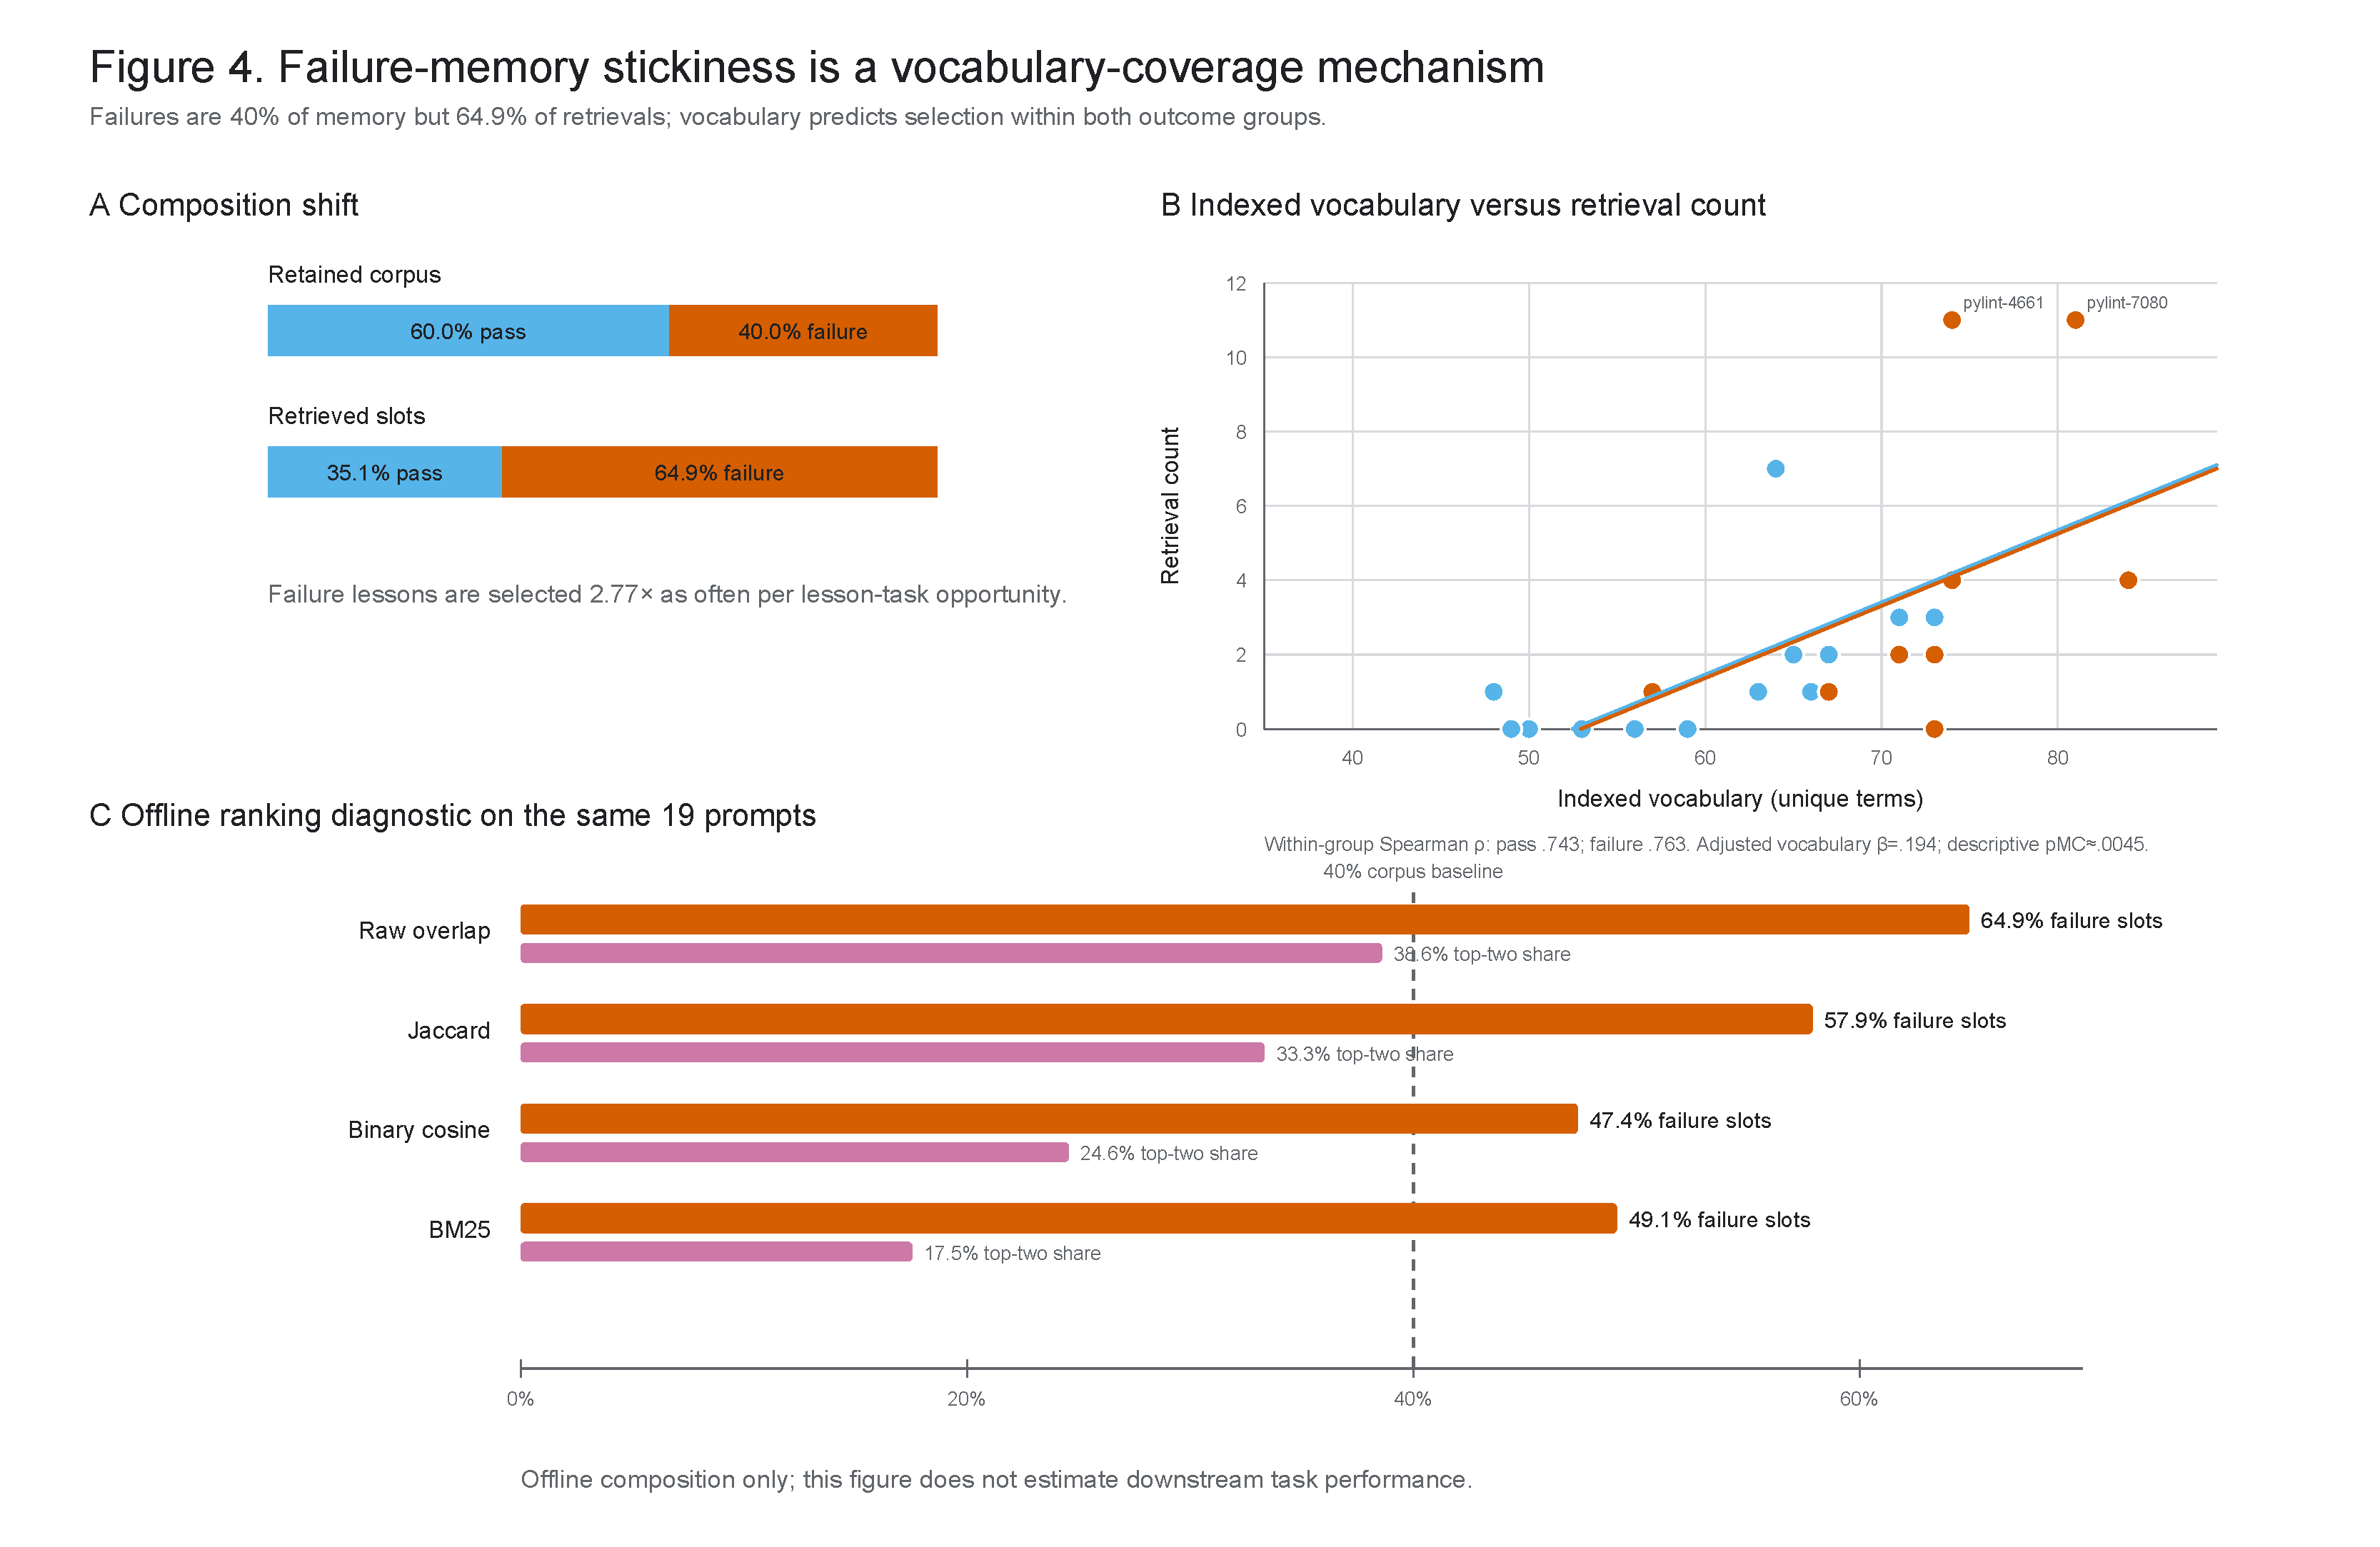
\includegraphics[width=0.85\textwidth]{figures/pdf/figure-4-failure-memory-stickiness.pdf}
\caption{\textbf{Failure-memory stickiness and lexical coverage.}
Hybrid's retained corpus was 40\% failure-derived, while failures
occupied 37/57 retrieval slots (64.9\%). Retrieval count increased with
indexed vocabulary within both success and failure groups. Because
failure status plausibly acts through indexed vocabulary breadth, the
adjusted regression is a mechanism diagnostic rather than an attribution
of signal away from failure. It does not establish an effect on held-out
score.}
\label{fig:4}
\end{figure*}

\subsection{Capacity saturation}\label{capacity-saturation}

Hybrid Pack source grew from 7,053 to 62,506 bytes. Generation 25 first
exceeded the 64,000-byte policy and succeeded after one repair. Every
candidate in generations 26 through 28 remained over the cap after four
author or repair requests; the closest final candidate was 65,928 bytes.
Mean authoring requests rose from 1.0 over the first five generations to
3.2 over the last five, and mean authoring cost rose from \$0.249 to
\$2.114.

The policy rejection and retained-state plateau directly establish
policy-cap saturation under this append-oriented design. Task identity
and difficulty are confounded with generation order, so the cost trend
is descriptive. The result does not establish a general limitation of
ActiveGraph or executable memory.

\begin{figure*}[!t]
\centering
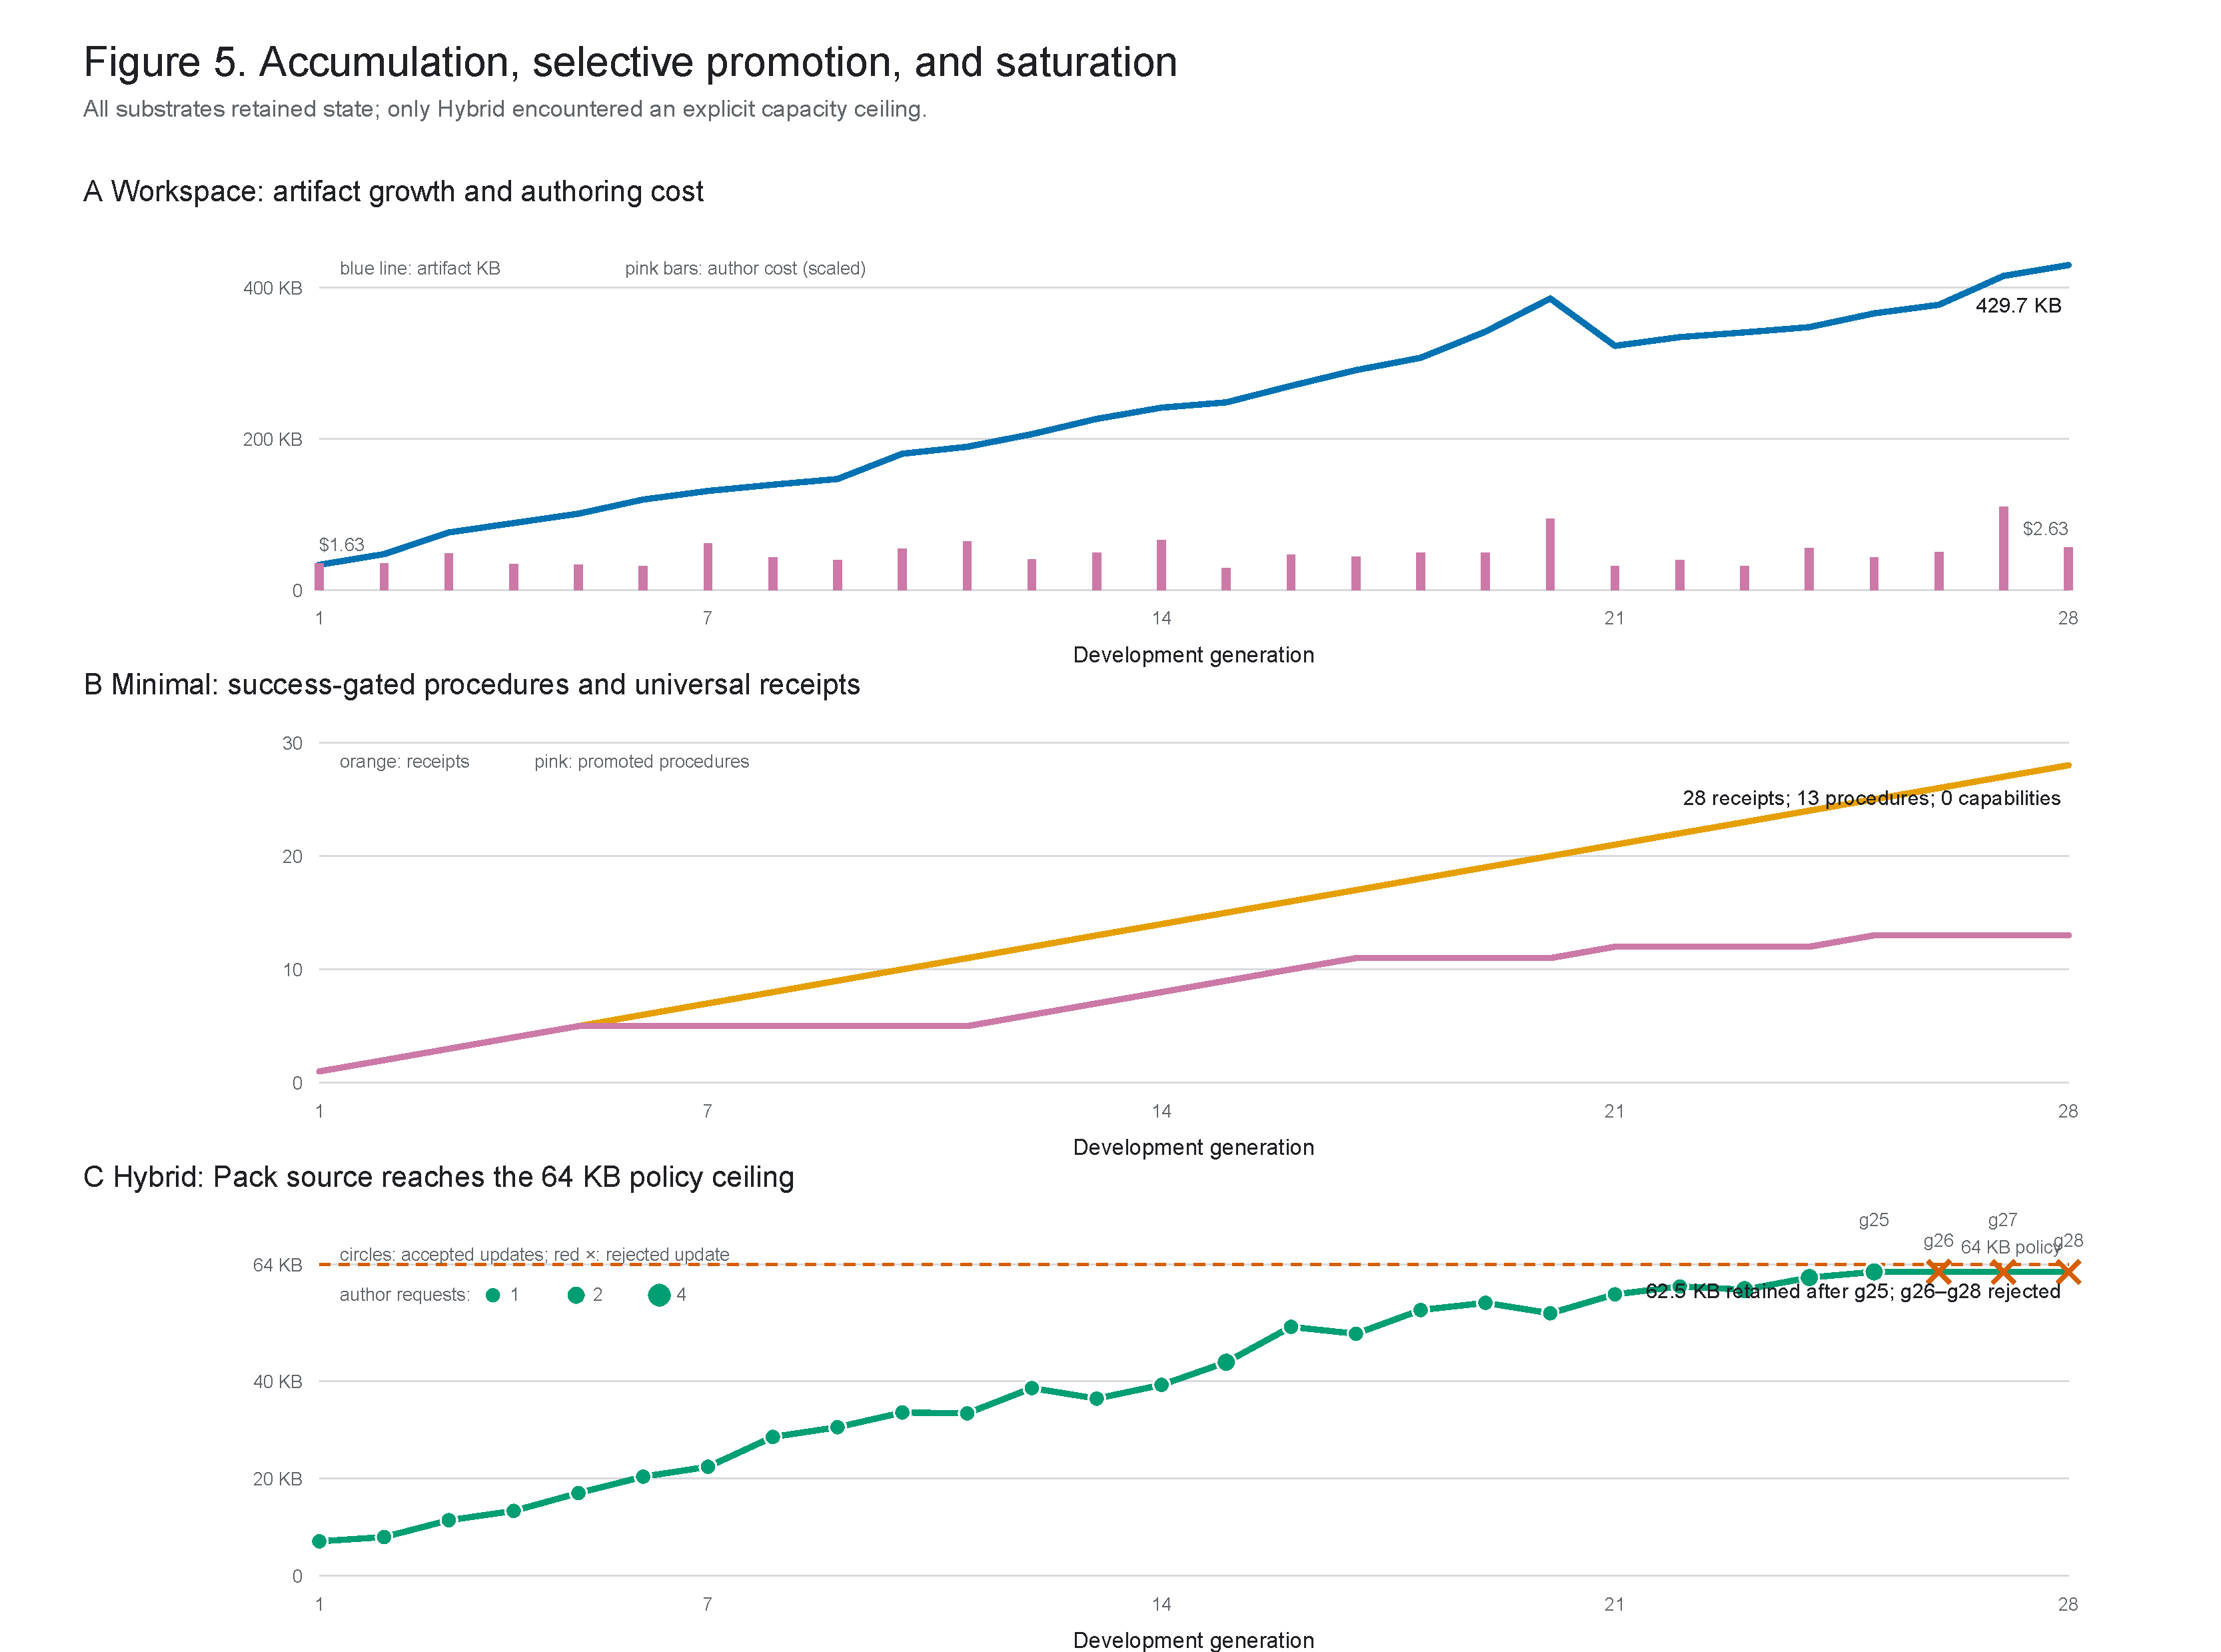
\includegraphics[width=0.85\textwidth]{figures/pdf/figure-5-accumulation-saturation.pdf}
\caption{\textbf{Accumulation, rising effort, and saturation.} Panel A
shows Workspace artifact growth and authoring cost; panel B shows
Minimal's universal receipts and success-gated procedures; panel C shows
Hybrid Pack growth and rejected updates at the 64,000-byte source
policy. Hybrid generation 25 succeeded after repair and generations 26
through 28 produced no within-cap candidate. The cost trend is
descriptive because generation order is confounded with task identity
and difficulty.}
\label{fig:5}
\end{figure*}

\subsection{Update-proposal taxonomy}\label{update-proposal-taxonomy}

A frozen codebook was applied to all 84 generation-level reflection
proposals. Each coder saw opaque shuffled excerpts without architecture,
task, sequence, score, acceptance, cost, or later retrieval metadata.
Sol and Terra completed separately executed, outcome-blind coding passes
using different model families. Sol also generated the proposals it
later coded; Terra did not. Original labels were hashed before
comparison and no disagreement was adjudicated.

Both coders labeled 84/84 proposals as natural-language, append-only,
nonexecutable, operational guidance with no specified activation. They
agreed on failure specificity for 83/84 proposals and validation
strategy for 82/84. These replicated labels support a stable description
of proposal form.

Interpretive fields were less stable and remain exploratory. Their
complete agreement results and coder marginals appear in Appendix E.

The shared reflector therefore produced a homogeneous representational
genre. Configuration-specific gates selected different retained
mixtures: Minimal accepted 13 success-derived proposals and no
failure-derived proposals; Workspace accepted 25 proposals including 12
after failures; Hybrid accepted 25 including ten after failures. Human
inter-rater reliability remains pending. The 84/84 form agreement is a
cross-model consistency check, not independent human reliability. The
analysis describes common update proposals rather than every native
Workspace edit or Pack source change.

\section{Audited cases}\label{audited-cases}

Case selection followed a frozen rule that required a complete chain:

\begin{quote}
retained update -\textgreater{} expression -\textgreater{} plausible
mechanism -\textgreater{} later behavior
\end{quote}

The rule also required comparison with the exact task-specific range
among equivalent duplicates.

\textbf{Apparent success.} Workspace passed a held-out SymPy task. Its
retained SymPy lesson concerned a different mechanism, and a no-context
run generated essentially the same fix. Equivalent outcomes on the task
ranged from failure to pass. The receipts establish a pass and reject
the learned-transfer story.

\textbf{Apparent failure.} Hybrid scored 0.48 on quota scheduler after
retrieving mechanistically skewed lessons. Six equivalent no-context
runs on the same task ranged from 0.48 to 1.00. The evolved score
equaled the observed minimum. The receipts establish retrieval skew and
reject attribution of this outcome to that skew.

\textbf{Outside-range regression.} Minimal failed a scikit-learn task
that all six equivalent no-context runs passed. The retained-context
trajectory changed an algorithm and rewrote an established
expected-output test. The ablation made a smaller fix and passed the
restored official test. This is consistent with harmful behavioral
mediation in that trace. Across all 57 configuration-task cases,
however, one outside-range result was observed against a tie-aware
conditional expectation of 1.71, so the case is not a population or
chance detection. The trace does not identify one retained sentence as
the cause.

\textbf{Capacity ceiling.} Hybrid generation 25 succeeded after a repair
near the policy cap. Generations 26 through 28 produced four over-cap
candidates each. This case establishes a direct mechanism from
append-only accumulation to failed retention.

Together, the cases show why receipts must be permitted to invalidate
stories in both directions. They also show why score, mechanism, and
attribution should be reported separately.

\FloatBarrier

\section{Related work}\label{related-work}

Self-improving agent systems measure different portions of the
five-construct chain. STOP reports repeated recursive improver
optimization and held-out task utilities. Gödel Agent
\citep{yin2024godel} evaluates runtime self-referential modification
with tool and policy ablations. SICA optimizes a coding-agent source
tree through a reported primary lineage. Darwin Gödel Machine uses a
branching archive and reports transfer across benchmarks, models, and
languages. Huxley-Gödel Machine explicitly measures descendant
productivity through clade-metaproductivity.

Our study complements these capability results by instrumenting
retained-state attribution. Table 6 separates unevolved baselines,
mechanism interventions, independent complete evolution runs, versioned
provenance, immutable exposure receipts, and recursive-improvement
operationalization. No design reports every listed feature. This study
lacks independent evolution-lineage replication and does not identify
descendant productivity. It adds sham state, initial-request duplicates,
and immutable exposure receipts to a persistent post-curriculum
comparison.

Reflexion \citep{shinn2023reflexion} shows that episodic linguistic
feedback can alter later trials; AI Agents That Matter
\citep{kapoor2024agents} motivates cost, holdout, and attribution
controls. Stochasticity in Agentic Evaluations
\citep{mustahsan2025stochasticity} motivates consistency analysis; PACE
\citep{shawn2026pace} studies noisy acceptance. Useful Memories Become
Faulty When Continuously Updated by LLMs \citep{zhang2026faulty}
contrasts episodes with consolidation; DeltaMem \citep{tan2026deltamem}
studies residual-tree memory. Together they motivate measurement of
retained-state mechanisms.

The closest conceptual precedents come from three adjacent traditions.
Memory evaluation distinguishes stored, retrieved, selected, and
utilized material; causal mediation separates intervention, mediator,
trajectory, and outcome; systems provenance and observability bind
events without by themselves identifying causal effects. Our residual
contribution is to unify these distinctions for persistent
self-modification, keep descendant productivity as a separate recursive
endpoint, profile expression across heterogeneous retained substrates,
and bind configuration-specific claims to receipts and actor-visible
controls. The framework is a domain-specific evidentiary synthesis
rather than a claim that each component is unprecedented.

\textbf{Table 6: Related-work evidence features.} ``Yes'' means that the
cited primary paper reports the feature. ``Partial'' identifies a nearby
but weaker design. ``NR'' means not reported and does not imply that the
authors could not implement it. Cells were re-audited against the linked
primary paper versions on 2026-07-23. The strict receipt column requires
immutable binding among retained state, evaluation exposure, trajectory,
and outcome.

\setcounter{table}{5}
\begin{landscape}
\begin{table*}[p]
\caption{Author-classified related-work evidence features based on primary papers read on 2026-07-23. NR means not reported and is not independently verified here.}
\label{tab:related}
\centering\scriptsize
\setlength{\tabcolsep}{3pt}
\textbf{Panel A: substrate, transfer, and interventions}\\[2pt]
\begin{tabularx}{\linewidth}{@{}lX X X X X@{}}
\toprule
\textbf{System} & \textbf{Retained surface} & \textbf{Held-out transfer} & \textbf{Initial baseline} & \textbf{Mechanism intervention} & \textbf{Sham state}\\
\midrule
STOP \cite{zelikman2023stop} & Python improver/scaffold & Yes: independent LPN and five new utilities & Seed improver & Nonrecursive and alternative improvers & NR\\
G{\"o}del Agent \cite{yin2024godel} & Runtime logic/actions & Partial: held-out splits & Initial policy and manual baselines & Initial-tool ablations & NR\\
SICA \cite{robeyns2025sica} & Coding-agent source tree & NR: utility reused in primary run & Initial agent & NR & NR\\
DGM \cite{zhang2025dgm} & Coding-agent branching archive & Cross-benchmark, model, language & Initial agent and manual baselines & Without self-improvement/open exploration & NR\\
HGM \cite{wang2025hgm} & Coding-agent search tree & Benchmark and model transfer & Shared initial agent & Matched SICA/DGM selection & NR\\
This study & Workspace; procedures/receipts; Pack & 19 disjoint post-curriculum tasks & Cold floor and initial harness & Partial: state hash preserved; actor-visible ablation collapses with cold & Opaque sham; mismatch reported\\
\bottomrule
\end{tabularx}
\vspace{8pt}

\textbf{Panel B: replication, provenance, and recursive-improvement evidence}\\[2pt]
\begin{tabularx}{\linewidth}{@{}lX X X X X@{}}
\toprule
\textbf{System} & \textbf{Complete evolution runs} & \textbf{Identical initial-request duplicates} & \textbf{Versioned lineage/provenance} & \textbf{Immutable exposure/trajectory receipts} & \textbf{Descendant productivity}\\
\midrule
STOP & Five GPT-4; 25 smaller-model in key experiments & NR & NR & NR & NR\\
G{\"o}del Agent & Six cycles per task & NR & NR & NR & NR\\
SICA & NR: one primary lineage & NR & Yes: archive of agents/results & NR & NR\\
DGM & Three complete runs in stability analysis & NR & Traceable archive tree & NR & NR\\
HGM & NR for repeated complete searches & NR & Retained search tree & NR & Yes: clade-metaproductivity\\
This study & No: one lineage per configuration & Six labels per task & Immutable generations/hashes & State, exposure, request, trajectory, grader, adjudication & No: not identified\\
\bottomrule
\end{tabularx}
\end{table*}
\end{landscape}

\clearpage

\section{Discussion}\label{discussion}

The frozen null does not establish that persistent self-modification
cannot improve agents. It establishes that three retained
configurations, under one common interface and one lineage each, did not
meet the specified uplift criterion. The mechanism audit explains why a
score-only summary would discard the most informative evidence.

First, native update breadth and evaluation-time expression are separate
design dimensions. Workspace retained arbitrary files, Minimal retained
procedures and receipts, and Hybrid retained executable Pack source. The
actor received truncated static text, complete static text, or
task-conditioned text. It received no callable retained capability.
Evaluation therefore compared native substrates after a consequential
common transformation.

Second, proposal, acceptance, retrieval, and expression form a pipeline.
The common reflector produced one representational genre across all 84
proposals. Acceptance gates created different epistemic mixtures.
Workspace and Hybrid retained failure-derived proposals that Minimal
excluded. Hybrid's lexical retriever then concentrated exposure on
broad-vocabulary failure lessons. Each mechanism belongs inside the
system boundary because each changes what a later actor can use.

Third, control labels can collapse or confound contrasts. Cold and the
nominal state-hidden ablation preserved different provenance but
delivered the same actor-visible intervention, so the frozen
single-ablation comparison is one draw from the no-context distribution.
Pooled-six and leave-one-ablation-out sensitivities preserve the null.
The opaque sham matched evolved bytes for Workspace and Minimal but not
Hybrid, and it differed in tokenization and semantic load. Equivalent
duplicates varied despite identical first requests. A positive
evolved-minus-sham contrast can therefore combine useful expression,
possible sham interference, and ordinary outcome spread. The control
ladder makes these alternatives explicit and suggests the next
diagnostic comparison.

Fourth, append-only retention carries a measurable maintenance burden.
Hybrid reached a hard cap; Workspace and Minimal accumulated without
consolidation. This observation motivates consolidation, pruning, and
replacement as first-class update operations. It does not establish
which operation would improve held-out performance.

The instruments are directly applicable in principle to persistent
agents whose retained-state inventory, eligibility rule, adapter
emissions, and actor-visible actions can be frozen and inspected.
Systems without byte-copy semantics should declare a computable proxy or
mark the byte axes not applicable. Equivalent duplicates can be retained
whenever multiple labels issue byte-identical initial requests under a
common execution contract. The control ladder can be selected according
to the intended causal claim. The update-proposal taxonomy can be
applied to shared reflectors while native state changes are analyzed
separately. Receipts can bind retained artifacts, exposures,
trajectories, graders, and adjudication.

\section{Limitations}\label{limitations}

The study completed one development lineage per configuration. The six
equivalent labels expose outcome variability and do not replace
independent evolution replications. All configurations shared one model
and outer agent, which may dominate configuration differences. The
held-out families contained ten, six, and three tasks. ActiveGraph
uncertainty estimates are especially unstable.

Cold and cold ablation were actor-visible-equivalent. Although cold
ablation validated a lineage state hash, it provided no lineage-derived
input, tool, workspace, instruction, or later protocol difference. The
frozen primary contrast is therefore not a separable matched-lineage
intervention. Pooled and leave-one-ablation-out sensitivities use the
available equivalent controls but do not create independent
evolution-lineage replication.

The common interface constrained native expression and exposed no
retained interactive capability. This limits architecture ranking and
creates the expression bottleneck examined in the paper. A general
auditability-expressivity relationship requires an intervention that
varies the interface while holding retained state fixed.

The sham targeted byte matching rather than token or semantic matching,
and Hybrid retained a substantial byte-size mismatch. It remains useful
as an interference control and cannot identify equal-compute semantic
effects. Duplicate-label pairwise gaps are dependent and post-hoc. The
task-level ranges are descriptive.

The update-proposal taxonomy used two language-model coders, one of
which also generated the proposals it coded. Exact agreement on
representational form is a cross-model consistency check and does not
substitute for independent human coding. Interpretive labels showed
lower exact agreement and remain exploratory. Configuration masking may
be incomplete because proposal form can reveal substrate.

The retrieval analysis identifies lexical selection mechanics and does
not establish causal harm to score. Offline re-ranking produced no new
behavioral outcomes. No retrieval-harm experiment or consolidation
intervention is part of this study.

The local ActiveGraph benchmark and the Hybrid Pack share author-built
technology. Sealed checks and an observed result unfavorable to Hybrid
reduce a simple directional-bias concern but do not remove the
structural conflict.

\section{Conclusion}\label{conclusion}

All three recorded configurations retained persistent changes. Their
evaluation interface expressed those changes mainly as text, their
controls exhibited substantial outcome spread and left interference
uncontrolled, and none met the frozen uplift criterion. The resulting
null separates five claims that are often compressed into one:
retention, expression, behavioral mediation, task improvement, and
recursive improvement.

The central lesson is operational. Treat reflection templates,
acceptance gates, retrievers, adapters, execution paths, and controls as
components of the self-improving system. Measure each link with receipts
and matched interventions. In the studied system, the interface and
acceptance mechanism substantially determine which retained
modifications can be admitted, expressed, and evaluated.

\paragraph{Artifact availability.} The version-controlled release includes the paper, generated tables, frozen coding artifacts, figures, audit scripts, and a self-verifying manifest. Complete trace archive DOI pending its separate disclosure scan and deposit.

\clearpage
\balance
\bibliographystyle{unsrt}
\bibliography{references}
\clearpage
\nobalance
\appendix

\section{Adjudication sensitivity}\label{a.-adjudication-sensitivity}

The raw run contained 215 immediately valid rows and 13 rows requiring
policy adjudication. The final dataset retained all 228 attempts.
Categories were six official SWE task timeouts, six Terminal
agent-budget timeouts with completed zero verifiers, and one ActiveGraph
snapshot contradiction resolved by a sealed grader-only retry of the
hash-identical submission.

Eight of nine frozen \texttt{evolved\ -\ cold\ ablation} contrasts are
identical when raw invalid rows are scored zero and when the frozen
adjudication decisions are applied. The exception is Hybrid ActiveGraph:
the contrast moves from -26.0 points under raw-invalid-as-zero to -10.0
points after the hash-identical quota-scheduler regrade. It remains
negative and the frozen conclusion is unchanged. A raw complete-case
analysis gives +7.3 points for this cell because it drops the evolved
invalid row. Complete-case contrasts are reported only as sensitivity
analyses because dropping bounded failures changes the estimand and can
favor arms with more invalid outcomes.

The study's single adjudication judgment moved a score in the evolved
arm's favor, and the frozen conclusion remained null.

Machine-readable table:
\path{data/generated/adjudication-sensitivity.csv}

\section{Timeout taxonomy}\label{b.-timeout-taxonomy}

\begin{table*}[t]
\caption{Timeout and adjudication taxonomy.}
\label{tab:timeouts}
\centering\small
\begin{tabularx}{\textwidth}{@{}l r X X@{}}
\toprule
\textbf{Category} & \textbf{Count} & \textbf{Treatment} & \textbf{Interpretation}\\
\midrule
Official SWE task timeout & 6 & Scored zero & Official evaluation exceeded the frozen 3,600-second task limit.\\
Terminal agent-budget timeout & 6 & Scored zero & Agent exhausted 1,800 seconds and the completed verifier returned zero.\\
ActiveGraph snapshot regrade & 1 & Hash-identical grader-only retry & Original grader contradicted a receipt-bound parsable submission; no model action was rerun.\\
\bottomrule
\end{tabularx}
\end{table*}

Timeouts remain outcomes under the bounded-agent estimand. The taxonomy
separates agent budget exhaustion, official evaluator limits, and
infrastructure contradiction.

\section{Success-conditional efficiency}\label{c.-success-conditional-efficiency}

For the binary SWE and Terminal families, the companion table reports
mean cost and wall time among successful attempts for every architecture
and arm: \path{data/generated/success-conditional-efficiency.csv}.

These quantities describe the resource profile of observed successes.
They do not estimate causal efficiency because conditioning on success
selects different tasks and trajectories across arms. Unconditional
costs remain the primary resource comparison.

\section{Provenance}\label{d.-provenance}

The study specification is \texttt{research/local\_study.json}, SHA-256
\texttt{8313d219\allowbreak{}71452704\allowbreak{}893200d2\allowbreak{}022718fe\allowbreak{}ca985142\allowbreak{}ae32fe7d\allowbreak{}16932d34\allowbreak{}a0e0d581},
with frozen status at study commit
\texttt{55984389\allowbreak{}4578141d\allowbreak{}fbd39b7b\allowbreak{}ae2246db\allowbreak{}76e57bde}
dated 2026-07-17T18:30:38-07:00. The compact release does not retain an
independently witnessed timestamp for the first development call. The
Round 1 manuscript package was commit
\texttt{8bdff502\allowbreak{}cc08be96\allowbreak{}8b21bbe5\allowbreak{}ebf177d4\allowbreak{}9879a0fb}.

The provenance manifest records byte counts and SHA-256 hashes for the
paper package's frozen analytical datasets and reports, adjudication
ledger, post-hoc metrics, masked coding packet, both original coder
label files, agreement report, and manuscript:
\path{provenance-manifest.json}.

The adjudication ledger separately hashes each changed row and its
supporting evidence. Both original taxonomy-label files were frozen
before adjudication.

\section{Cross-model coding agreement}\label{e.-cross-model-coding-agreement}

The table reports exact agreement, Cohen's kappa, and Gwet's AC1 for two
separately executed, outcome-blind model-coding passes using different
model families. Sol generated the 84 proposals it later coded; Terra
supplied the other pass. The analysis is therefore a cross-model
consistency check rather than independent human reliability. Kappa is
undefined when both coders use one category for every item because the
marginals have zero variance. AC1 is a supplemental prevalence-robust
coefficient computed with the full pre-specified category vocabulary.
Its value of 1.000 for invariant fields is mechanical and supplies no
evidence beyond 84/84 exact agreement.

\begin{table*}[t]
\caption{Cross-model coding consistency. Sol generated the proposals it coded; undefined kappa indicates zero marginal variance.}
\label{tab:coding-agreement}
\centering\scriptsize
\begin{tabular}{@{}lrrr@{}}
\toprule
\textbf{Field} & \textbf{Exact agreement} & \textbf{Cohen's kappa} & \textbf{Gwet's AC1}\\
\midrule
Primary update target & 76/84 (90.5\%) & 0.000 & 0.904\\
Secondary update target & 47/84 (56.0\%) & -0.081 & 0.543\\
Representational form & 84/84 (100\%) & undefined & 1.000\\
Transfer scope & 63/84 (75.0\%) & 0.470 & 0.717\\
Abstraction level & 59/84 (70.2\%) & 0.529 & 0.647\\
Evidence grounding & 59/84 (70.2\%) & 0.428 & 0.669\\
Failure specificity & 83/84 (98.8\%) & 0.661 & 0.988\\
Validation strategy & 82/84 (97.6\%) & 0.592 & 0.976\\
Consolidation operation & 84/84 (100\%) & undefined & 1.000\\
Executable status & 84/84 (100\%) & undefined & 1.000\\
Anticipated activation & 84/84 (100\%) & undefined & 1.000\\
Counterfactual actionability & 84/84 (100\%) & undefined & 1.000\\
Novelty relative to prior state & 84/84 (100\%) & undefined & 1.000\\
Confidence & 63/84 (75.0\%) & 0.393 & 0.687\\
\bottomrule
\end{tabular}
\end{table*}

For primary update target, Sol assigned 76 procedure and eight
validation-asset labels, while Terra assigned all 84 to procedure. The
resulting confusion is 76 procedure/procedure and eight
validation-asset/procedure cases, which explains 90.5\% exact agreement
with kappa 0.000. Complete coder marginals and disagreements are
retained in \path{data/taxonomy/coder-agreement.json}.

No coefficient interval is reported because these are two fixed
model-coding passes used as a prompt and model-sensitivity check rather
than sampled human raters. Interpretive fields remain exploratory.

\section{Actor-visible control-collapse sensitivity}\label{f.-actor-visible-control-collapse-sensitivity}

Source inspection confirms that cold and cold ablation use the same
task, model, seed field, tools, workspace, system instructions, empty
retained-context field, and later actor-visible tool protocol. Cold
ablation validates the lineage state hash before suppressing its
contents; that provenance difference never reaches the actor. The frozen
\texttt{evolved\ -\ cold\ ablation} contrast is therefore retained as a
decision record, not described as a separable lineage intervention.

The pooled-six and leave-the-matched-ablation-out calculations use only
the committed compact score table. Across Workspace, Minimal, and
Hybrid, the pooled-six deltas are +6.7, -3.3, and +6.7 points for SWE;
+11.1, -22.2, and -5.6 for Terminal; and -9.9, +4.1, and -9.9 for
ActiveGraph. The corresponding leave-one-out deltas are +8.0, -6.0,
+6.0; +10.0, -20.0, -6.7; and -8.4, +3.2, -9.9 points. The frozen
no-uplift decision is unchanged.

A tie-aware conditional exchangeability calculation pools each evolved
score with its six actor-visible-equivalent controls and uniformly
relabels the focal score. Only a unique minimum or maximum is strictly
outside the other six. Across 57 configuration-task cases, the expected
outside-range count is 12/7 (1.71) and the observed count is one. The
expected counts are 1/7 among 36 cases on stable control tasks and 11/7
among 21 cases on variable control tasks. Machine-readable outputs are
\path{data/generated/equivalent-control-sensitivity.csv} and
\path{data/generated/outside-range-exchangeability.json}.

\end{document}
